%%
% Copyright (c) 2017 - 2024, Pascal Wagler;
% Copyright (c) 2014 - 2024, John MacFarlane
%
% All rights reserved.
%
% Redistribution and use in source and binary forms, with or without
% modification, are permitted provided that the following conditions
% are met:
%
% - Redistributions of source code must retain the above copyright
% notice, this list of conditions and the following disclaimer.
%
% - Redistributions in binary form must reproduce the above copyright
% notice, this list of conditions and the following disclaimer in the
% documentation and/or other materials provided with the distribution.
%
% - Neither the name of John MacFarlane nor the names of other
% contributors may be used to endorse or promote products derived
% from this software without specific prior written permission.
%
% THIS SOFTWARE IS PROVIDED BY THE COPYRIGHT HOLDERS AND CONTRIBUTORS
% "AS IS" AND ANY EXPRESS OR IMPLIED WARRANTIES, INCLUDING, BUT NOT
% LIMITED TO, THE IMPLIED WARRANTIES OF MERCHANTABILITY AND FITNESS
% FOR A PARTICULAR PURPOSE ARE DISCLAIMED. IN NO EVENT SHALL THE
% COPYRIGHT OWNER OR CONTRIBUTORS BE LIABLE FOR ANY DIRECT, INDIRECT,
% INCIDENTAL, SPECIAL, EXEMPLARY, OR CONSEQUENTIAL DAMAGES (INCLUDING,
% BUT NOT LIMITED TO, PROCUREMENT OF SUBSTITUTE GOODS OR SERVICES;
% LOSS OF USE, DATA, OR PROFITS; OR BUSINESS INTERRUPTION) HOWEVER
% CAUSED AND ON ANY THEORY OF LIABILITY, WHETHER IN CONTRACT, STRICT
% LIABILITY, OR TORT (INCLUDING NEGLIGENCE OR OTHERWISE) ARISING IN
% ANY WAY OUT OF THE USE OF THIS SOFTWARE, EVEN IF ADVISED OF THE
% POSSIBILITY OF SUCH DAMAGE.
%%

%%
% This is the Eisvogel pandoc LaTeX template.
%
% For usage information and examples visit the official GitHub page:
% https://github.com/Wandmalfarbe/pandoc-latex-template
%%

% Options for packages loaded elsewhere
\PassOptionsToPackage{unicode}{hyperref}
\PassOptionsToPackage{hyphens}{url}
\PassOptionsToPackage{dvipsnames,svgnames,x11names,table}{xcolor}
%
\documentclass[
  paper=a4,
  ,captions=tableheading
]{scrartcl}
\usepackage{amsmath,amssymb}
% Use setspace anyway because we change the default line spacing.
% The spacing is changed early to affect the titlepage and the TOC.
\usepackage{setspace}
\setstretch{1.2}
\usepackage{iftex}
\ifPDFTeX
  \usepackage[T1]{fontenc}
  \usepackage[utf8]{inputenc}
  \usepackage{textcomp} % provide euro and other symbols
\else % if luatex or xetex
  \usepackage{unicode-math} % this also loads fontspec
  \defaultfontfeatures{Scale=MatchLowercase}
  \defaultfontfeatures[\rmfamily]{Ligatures=TeX,Scale=1}
\fi
\usepackage{lmodern}
\ifPDFTeX\else
  % xetex/luatex font selection
\fi
% Use upquote if available, for straight quotes in verbatim environments
\IfFileExists{upquote.sty}{\usepackage{upquote}}{}
\IfFileExists{microtype.sty}{% use microtype if available
  \usepackage[]{microtype}
  \UseMicrotypeSet[protrusion]{basicmath} % disable protrusion for tt fonts
}{}
\makeatletter
\@ifundefined{KOMAClassName}{% if non-KOMA class
  \IfFileExists{parskip.sty}{%
    \usepackage{parskip}
  }{% else
    \setlength{\parindent}{0pt}
    \setlength{\parskip}{6pt plus 2pt minus 1pt}}
}{% if KOMA class
  \KOMAoptions{parskip=half}}
\makeatother
\usepackage{xcolor}
\definecolor{default-linkcolor}{HTML}{A50000}
\definecolor{default-filecolor}{HTML}{A50000}
\definecolor{default-citecolor}{HTML}{4077C0}
\definecolor{default-urlcolor}{HTML}{4077C0}
\usepackage[top=1in,bottom=1in]{geometry}
\usepackage{longtable,booktabs,array}
\usepackage{calc} % for calculating minipage widths
% Correct order of tables after \paragraph or \subparagraph
\usepackage{etoolbox}
\makeatletter
\patchcmd\longtable{\par}{\if@noskipsec\mbox{}\fi\par}{}{}
\makeatother
% Allow footnotes in longtable head/foot
\IfFileExists{footnotehyper.sty}{\usepackage{footnotehyper}}{\usepackage{footnote}}
\makesavenoteenv{longtable}
% add backlinks to footnote references, cf. https://tex.stackexchange.com/questions/302266/make-footnote-clickable-both-ways
\usepackage{footnotebackref}
\usepackage{graphicx}
\makeatletter
\newsavebox\pandoc@box
\newcommand*\pandocbounded[1]{% scales image to fit in text height/width
  \sbox\pandoc@box{#1}%
  \Gscale@div\@tempa{\textheight}{\dimexpr\ht\pandoc@box+\dp\pandoc@box\relax}%
  \Gscale@div\@tempb{\linewidth}{\wd\pandoc@box}%
  \ifdim\@tempb\p@<\@tempa\p@\let\@tempa\@tempb\fi% select the smaller of both
  \ifdim\@tempa\p@<\p@\scalebox{\@tempa}{\usebox\pandoc@box}%
  \else\usebox{\pandoc@box}%
  \fi%
}
% Set default figure placement to htbp
% Make use of float-package and set default placement for figures to H.
% The option H means 'PUT IT HERE' (as  opposed to the standard h option which means 'You may put it here if you like').
\usepackage{float}
\floatplacement{figure}{H}
\makeatother
\setlength{\emergencystretch}{3em} % prevent overfull lines
\providecommand{\tightlist}{%
  \setlength{\itemsep}{0pt}\setlength{\parskip}{0pt}}
\setcounter{secnumdepth}{-\maxdimen} % remove section numbering
\ifLuaTeX
\usepackage[bidi=basic]{babel}
\else
\usepackage[bidi=default]{babel}
\fi
\babelprovide[main,import]{english}
% get rid of language-specific shorthands (see #6817):
\let\LanguageShortHands\languageshorthands
\def\languageshorthands#1{}
\makeatletter
\@ifpackageloaded{subfig}{}{\usepackage{subfig}}
\@ifpackageloaded{caption}{}{\usepackage{caption}}
\captionsetup[subfloat]{margin=0.5em}
\AtBeginDocument{%
\renewcommand*\figurename{Figura}
\renewcommand*\tablename{Tabla}
}
\AtBeginDocument{%
\renewcommand*\listfigurename{Lista de Figuras}
\renewcommand*\listtablename{Lista de Tablas}
}
\newcounter{pandoccrossref@subfigures@footnote@counter}
\newenvironment{pandoccrossrefsubfigures}{%
\setcounter{pandoccrossref@subfigures@footnote@counter}{0}
\begin{figure}\centering%
\gdef\global@pandoccrossref@subfigures@footnotes{}%
\DeclareRobustCommand{\footnote}[1]{\footnotemark%
\stepcounter{pandoccrossref@subfigures@footnote@counter}%
\ifx\global@pandoccrossref@subfigures@footnotes\empty%
\gdef\global@pandoccrossref@subfigures@footnotes{{##1}}%
\else%
\g@addto@macro\global@pandoccrossref@subfigures@footnotes{, {##1}}%
\fi}}%
{\end{figure}%
\addtocounter{footnote}{-\value{pandoccrossref@subfigures@footnote@counter}}
\@for\f:=\global@pandoccrossref@subfigures@footnotes\do{\stepcounter{footnote}\footnotetext{\f}}%
\gdef\global@pandoccrossref@subfigures@footnotes{}}
\@ifpackageloaded{float}{}{\usepackage{float}}
\floatstyle{ruled}
\@ifundefined{c@chapter}{\newfloat{codelisting}{h}{lop}}{\newfloat{codelisting}{h}{lop}[chapter]}
\floatname{codelisting}{Listing}
\newcommand*\listoflistings{\listof{codelisting}{Listas del Documento}}
\makeatother
\usepackage{bookmark}
\IfFileExists{xurl.sty}{\usepackage{xurl}}{} % add URL line breaks if available
\urlstyle{same}
\hypersetup{
  pdftitle={Gestión de Requerimientos JEP},
  pdfauthor={Versión actual: 1.7092a66 - clean - Mon, 25 Nov 2024 16:21:58 -0500},
  pdflang={en},
  pdfsubject={Implementación Proyecto},
  pdfkeywords={Integración, Interoperabilidad, JEP, Softgic},
  hidelinks,
  breaklinks=true,
  pdfcreator={LaTeX via pandoc with the Eisvogel template}}
\title{Gestión de Requerimientos JEP}
\usepackage{etoolbox}
\makeatletter
\providecommand{\subtitle}[1]{% add subtitle to \maketitle
  \apptocmd{\@title}{\par {\large #1 \par}}{}{}
}
\makeatother
\subtitle{Implementación Proyecto Evolución de Interoperabilidad JEP,
Softgic}
\author{Versión actual: 1.7092a66 - clean - Mon, 25 Nov 2024 16:21:58
-0500}
\date{2024-11-8}



%%
%% added
%%


%
% for the background color of the title page
%
\usepackage{pagecolor}
\usepackage{afterpage}

%
% break urls
%
\PassOptionsToPackage{hyphens}{url}

%
% When using babel or polyglossia with biblatex, loading csquotes is recommended
% to ensure that quoted texts are typeset according to the rules of your main language.
%
\usepackage{csquotes}

%
% captions
%
\definecolor{caption-color}{HTML}{777777}
\usepackage[font={stretch=1.2}, textfont={color=caption-color}, position=top, skip=4mm, labelfont=bf, singlelinecheck=false, justification=raggedright]{caption}
\setcapindent{0em}

%
% blockquote
%
\definecolor{blockquote-border}{RGB}{221,221,221}
\definecolor{blockquote-text}{RGB}{119,119,119}
\usepackage{mdframed}
\newmdenv[rightline=false,bottomline=false,topline=false,linewidth=3pt,linecolor=blockquote-border,skipabove=\parskip]{customblockquote}
\renewenvironment{quote}{\begin{customblockquote}\list{}{\rightmargin=0em\leftmargin=0em}%
\item\relax\color{blockquote-text}\ignorespaces}{\unskip\unskip\endlist\end{customblockquote}}

%
% Source Sans Pro as the default font family
% Source Code Pro for monospace text
%
% 'default' option sets the default
% font family to Source Sans Pro, not \sfdefault.
%
\ifnum 0\ifxetex 1\fi\ifluatex 1\fi=0 % if pdftex
    \usepackage[default]{sourcesanspro}
  \usepackage{sourcecodepro}
  \else % if not pdftex
    \usepackage[default]{sourcesanspro}
  \usepackage{sourcecodepro}

  % XeLaTeX specific adjustments for straight quotes: https://tex.stackexchange.com/a/354887
  % This issue is already fixed (see https://github.com/silkeh/latex-sourcecodepro/pull/5) but the
  % fix is still unreleased.
  % TODO: Remove this workaround when the new version of sourcecodepro is released on CTAN.
  \ifxetex
    \makeatletter
    \defaultfontfeatures[\ttfamily]
      { Numbers   = \sourcecodepro@figurestyle,
        Scale     = \SourceCodePro@scale,
        Extension = .otf }
    \setmonofont
      [ UprightFont    = *-\sourcecodepro@regstyle,
        ItalicFont     = *-\sourcecodepro@regstyle It,
        BoldFont       = *-\sourcecodepro@boldstyle,
        BoldItalicFont = *-\sourcecodepro@boldstyle It ]
      {SourceCodePro}
    \makeatother
  \fi
  \fi

%
% heading color
%
\definecolor{heading-color}{RGB}{40,40,40}
\addtokomafont{section}{\color{heading-color}}
% When using the classes report, scrreprt, book,
% scrbook or memoir, uncomment the following line.
%\addtokomafont{chapter}{\color{heading-color}}

%
% variables for title, author and date
%
\usepackage{titling}
\title{Gestión de Requerimientos JEP}
\author{Versión actual: 1.7092a66 - clean - Mon, 25 Nov 2024 16:21:58
-0500}
\date{2024-11-8}

%
% tables
%

\definecolor{table-row-color}{HTML}{F5F5F5}
\definecolor{table-rule-color}{HTML}{999999}

%\arrayrulecolor{black!40}
\arrayrulecolor{table-rule-color}     % color of \toprule, \midrule, \bottomrule
\setlength\heavyrulewidth{0.3ex}      % thickness of \toprule, \bottomrule
\renewcommand{\arraystretch}{1.3}     % spacing (padding)


%
% remove paragraph indentation
%
\setlength{\parindent}{0pt}
\setlength{\parskip}{6pt plus 2pt minus 1pt}
\setlength{\emergencystretch}{3em}  % prevent overfull lines

%
%
% Listings
%
%


%
% header and footer
%
\usepackage[headsepline,footsepline]{scrlayer-scrpage}

\newpairofpagestyles{eisvogel-header-footer}{
  \clearpairofpagestyles
  \ihead*{
\includegraphics{include/jeplogo.jpg}}
  \chead*{}
  \ohead*{2024-11-8}
  \ifoot*{Versión actual: 1.7092a66 - clean - Mon, 25 Nov 2024 16:21:58
-0500}
  \cfoot*{}
  \ofoot*{\thepage}
  \addtokomafont{pageheadfoot}{\upshape}
}
\pagestyle{eisvogel-header-footer}



%%
%% end added
%%

\begin{document}

%%
%% begin titlepage
%%
\begin{titlepage}
\newgeometry{left=6cm}
\newcommand{\colorRule}[3][black]{\textcolor[HTML]{#1}{\rule{#2}{#3}}}
\begin{flushleft}
\noindent
\\[-1em]
\color[HTML]{5F5F5F}
\makebox[0pt][l]{\colorRule[360049]{1.3\textwidth}{4pt}}
\par
\noindent

{
  \setstretch{1.4}
  \vfill
  \noindent {\huge \textbf{\textsf{Gestión de Requerimientos JEP}}}
    \vskip 1em
  {\Large \textsf{Implementación Proyecto Evolución de Interoperabilidad
JEP, Softgic}}
    \vskip 2em
  \noindent {\Large \textsf{Versión actual: 1.7092a66 - clean - Mon, 25
Nov 2024 16:21:58 -0500}}
  \vfill
}


\textsf{2024-11-8}
\end{flushleft}
\end{titlepage}
\restoregeometry
\pagenumbering{arabic}

%%
%% end titlepage
%%

% \maketitle


\section{Contenido}\label{sec:contenido}

\begin{itemize}
\tightlist
\item
  \hyperref[informaciuxf3n-del-documento]{Información del Documento}
\item
  \hyperref[gestiuxf3n-de-trabajo-del-proyecto]{Gestión de Trabajo del
  Proyecto}
\item
  \hyperref[modelo-de-requerimientos-de-interoperabilidad-proyecto-jep]{Modelo
  de Requerimientos de Interoperabilidad Proyecto JEP}
\item
  \hyperref[modelo-de-despliegue-de-requerimientos-de-interoperabilidad-proyecto-jep]{Modelo
  de Despliegue de Requerimientos de Interoperabilidad Proyecto JEP}
\end{itemize}

\newpage

\section{Información del
Documento}\label{sec:informaciuxf3n-del-documento}

\subsection{Versión del Documento}\label{sec:versiuxf3n-del-documento}

\begin{quote}
\end{quote}

Versión Actual

1.7092a66 - clean - Mon, 25 Nov 2024 16:21:58 -0500

Versiones Anteriores

1.5fc7144 - Compilación para entrega - Mon, 25 Nov 2024 19:50:29 +0000

1.c17d6d1 - Compilación para entrega - Mon, 25 Nov 2024 19:41:40 +0000

1.32d8d21 - Compilación para entrega - Tue, 19 Nov 2024 22:04:18 +0000

1.4fdd500 - Compilación para entrega - Tue, 19 Nov 2024 21:58:36 +0000

\subsection{Realizado Por}\label{sec:realizado-por}

Sofgic.co

\subsection{Revisado Por}\label{sec:revisado-por}

Sofgic.co

\newpage

\section{Gestión de Trabajo del
Proyecto}\label{sec:gestiuxf3n-de-trabajo-del-proyecto}

\subsection{Modelo de Gestión de Requerimientos de
Integración}\label{sec:modelo-de-gestiuxf3n-de-requerimientos-de-integraciuxf3n}

\begin{quote}
Modelo de Implementación Proyecto JEP, 2024. Softgic. Propuesta modelo
de gestión y atención requerimientos de integración del proyecto de
servicios de integración JEP. Ver 0.1.37
\end{quote}

El ciclo de entrega de requerimientos inicia con la planeación macro de
los objetivos entregables del proyecto de integración organizados en el
tiempo (de septiembre a diciembre del 2024).

Los roles técnicos convierten estos objetivos macro en requerimientos
comprendidos por épicas, características e historias (o casos de uso) de
integración.

Los ingenieros convierten a su vez las historias en tareas entregables,
individuales y autónomas, de tipo tarea (UT), diseño (DIS), pruebas de
calidad (QA), análisis (AN), entrega continua (CI/CD), etc. Una vez los
ingenieros tengan esta división de trabajo en tareas pueden pasar a la
implementación mediante iteraciones (ver Modelo de Implementación del
Proyecto JEP).

Los requerimientos del proyecto JEP son procesados mediante el modelo de
producción descrito más adelante.

\begin{figure}
\centering
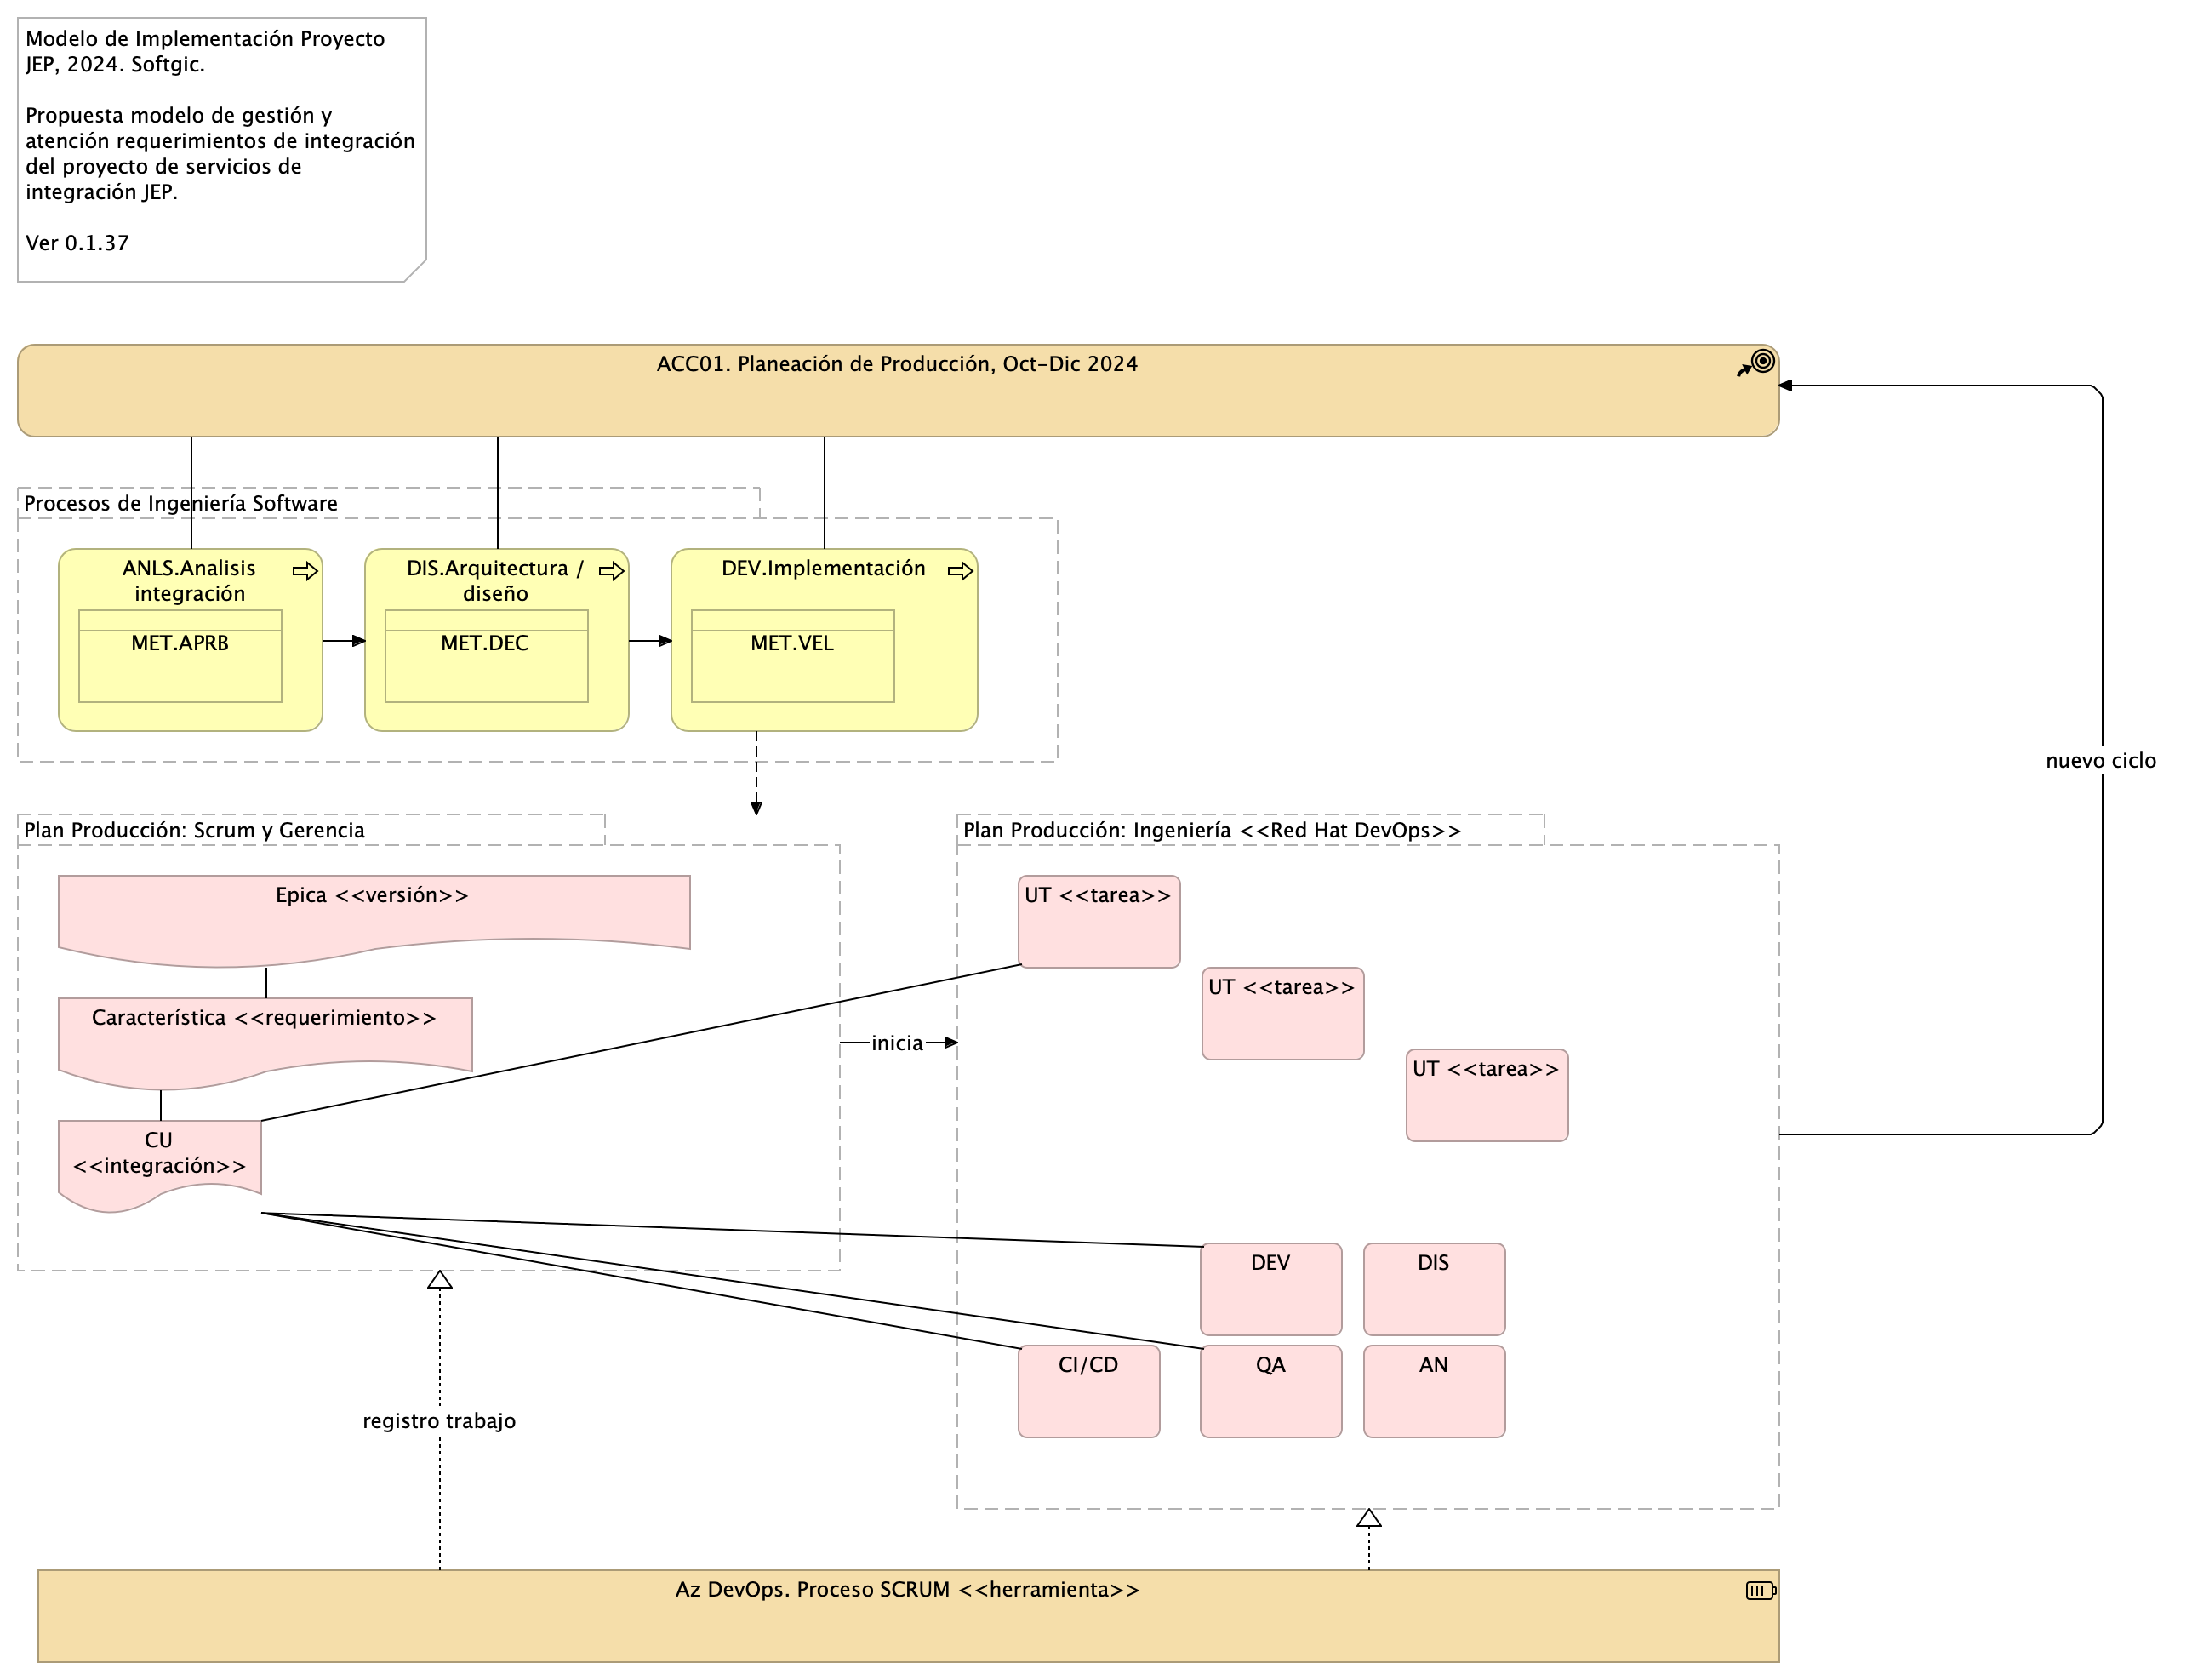
\includegraphics[width=\textwidth,height=5.20833in]{images/04.ING.2n.1a.Modelorequerimientos.png}
\caption{04.ING.2n.1a. Modelo requerimientos. \emph{Fuente: Repositorio
arquitectura Integración JEP
(2024)}}\label{fig:id-7c3abdaa8d9b46eebfd8f8e3e8d912ce}
\end{figure}

\subsubsection{Catálogo de
Elementos}\label{sec:catuxe1logo-de-elementos}

\begin{itemize}
\item
  \textbf{ACC01. Planeación de Producción, Oct-Dic 2024}. Objetivos y
  entregas en el tiempo, versiones de entrega del proyecto de
  integración.
\item
  \textbf{Procesos de Ingeniería Software}.
\item
  \textbf{ANLS.Analisis integración}. \#\#\# 2. ANSS (análisis).
\item
  Scrum, Funcional, Dueño producto cliente (requiere conocimiento del
  negocio).
\item
  Resultado: Refinamiento HU, modelo de negocio, es decir, diagrama de
  HU relacionadas unas con otras y con los conceptos de negocio en el
  repositorio de ARQ. Actualmente: no hay resultados de este proceso.
  Ejemplo del modelo de negocio
\end{itemize}

\subsubsection{Salidas}\label{sec:salidas}

\begin{itemize}
\tightlist
\item
  Modelo de negocio en el repo
\item
  Estimación --puede en devops
\item
  Análisis de dependencia en el repo
\end{itemize}

\subsubsection{KPI}\label{sec:kpi}

\begin{itemize}
\item
  Tasa de aprobación de HU por cliente Fuente: (Cantidad de HU refinadas
  y aprobadas por cliente {[}Repo Sharepoint{]} / Total de cantidad de
  HU {[}Azure DevOps{]}) Dato 26/10/2023: (30/44) = 0,68
\item
  Tasa de error en Bug por PR entregados Fuente: (Cantidad de solicitude
  de cambio en rama (Pull Reqst) de Correcciones (fix) o Regresión
  (reverts) {[}Bitbucket{]} / Cantidad total de PR desplegados
  {[}Bitbucket{]}) Dato 26/10/2023: (8/111)*100 = 7,2\%
\item
  \textbf{MET.APRB}. Cod. APRB Nombre indicador Tasa de aprobación de HU
  por cliente Uso Estabildad de requerimientos. Contensión del flujo de
  trabajo inicio de desarrolo Proceso ANLS Calculo de medición Cantidad
  de HU refinadas y aprobadas por cliente / Total de cantidad de HU
  Fuente {[}Repo Sharepoint{]}, {[}Azure DevOps{]})
\item
  \textbf{DIS.Arquitectura / diseño}. \#\#\# KPI
\item
  Nivel de HU sin detalle técnico Fuente: (Cantidad de HU refinadas y
  aprobadas sin diseño de implementacion {[}Repo Sharepoint{]} / Total
  de cantidad de HU {[}Azure DevOps{]}) Dato 26/10/2023: 0/44=0
\item
  \textbf{MET.DEC}. Cod.: DEC Nombre indicador: Decisiones de diseño,
  justificaciones, validaciones Uso: Estabildad de requerimientos.
  Control de alineación desarrollo-demanda Proceso: DIS Calculo de
  medición: Cantidad de HU refinadas y aprobadas por cliente / Total de
  cantidad de HU Fuente: {[}Repo Sharepoint{]}, {[}Azure DevOps{]})
\item
  \textbf{DEV.Implementación}. \#\#\# KPI
\item
  Velocidad de construcción Fuente: (Cantidad de puntos de HU ejecutadas
  {[}Azure DevOps{]} / Horas habiles del mes de trabajo {[}Calculo
  manual{]}) Dato 26/10/2023: 83 / 153 = 0,54 HU/horas
\item
  Tasa de cierre de defectos Fuente: (Cantidad de Bug solucionados
  {[}Azure DevOps{]} / Total de Bugs a corte sin nuevos {[}Azure
  DevOps{]}) Dato 26/10/2023: 81 / 920 = 0,088
\item
  Indice de dependecia de Lider Técnico Fuente: (Cantidad de actividades
  retrazadas semanales segun las HU planeadas / Total de HU planeadas
  para ejecución) Dato 26/10/2023: Pendiente proxima semana
\item
  \textbf{MET.VEL}. Cod. VEL Nombre indicador Velocidad de construcción
  Uso Capacidad interna de desarrollo Proceso DEV Calculo de medición
  Cantidad de puntos de HU ejecutadas / Horas habiles del mes de trabajo
  Fuente {[}Azure DevOps{]}, {[}Calculo manual{]}
\item
  \textbf{Plan Producción: Scrum y Gerencia}.
\item
  \textbf{Plan Producción: Ingeniería (Red Hat DevOps)}.
\item
  \textbf{UT (tarea)}. Unidad mínima de trabajo (tarea por
  desarrollador).
\item
  \textbf{UT (tarea)}. Unidad mínima de trabajo (tarea por
  desarrollador).
\item
  \textbf{UT (tarea)}. Unidad mínima de trabajo (tarea por
  desarrollador).
\item
  \textbf{DEV}. Alcance de QA unitaria
\item
  \textbf{CI/CD}. Actividades DevOps del ciclo o iteración de
  implementación.
\end{itemize}

\subsection{Modelo de Producción e Implementación de Integración
JEP}\label{sec:modelo-de-producciuxf3n-e-implementaciuxf3n-de-integraciuxf3n-jep}

\begin{quote}
Modelo de Producción e Implementación Proyecto JEP, 2024. Softgic.
Modelo de gestión y atención requerimientos de integración del proyecto
de integración JEP, 2024. Softgic. Relación con herramienta de gestión
Az DevOps. Ver 0.1.12
\end{quote}

El modelo de producción que procesa los requerimientos del proyecto JEP
inicia con la creación de un tramo de la planeación de la solución de
integración, esto es un ciclo de implementación o iteración del proyecto
de integración JEP.

(ING) Procesos de ingeniería. Arrancan los procesos mínimos de
ingeniería previos a la construcción de la integración.

(PRY) Planificación de historias de usuario. La porción de la planeación
de producción aprobada para la construcción se planifica en historias o
casos de uso, u cualquier otra forma de medición de avance.

(ING) Creación e inicio de iteraciones de implementación incremental. La
planificación de HU (CU, u otra) es tareificada y asignada a
desarrolladores disponibles. Además, las tareas asignadas son
organizadas en ciclos de trabajo fijo (iteraciones). Esta ejecución es
la línea de trabajo principal del proyecto JEP.

(PRY, ING) Coordinación de líneas de trabajo. Las entregas de la línea
de trabajo del proyecto JEP debe ser compasada con otras líneas de
trabajo de la JEP, con las que puede haber una relación de secuencia o
dependencia externa.

Durante la ejecución de la iteraciones determinadas, inicia nuevamente
el ciclo del proyecto desde la creación de un nuevo tramo de la
planeación de producción.

\subsubsection{Mapeo del Modelo con Herramienta de Registro del Trabajo
(az
devops)}\label{sec:mapeo-del-modelo-con-herramienta-de-registro-del-trabajo-az-devops}

\begin{itemize}
\tightlist
\item
  Épica = Versión de entrega de la solución como un todo
\item
  Característica = Requerimiento de integración, del cual pueden
  desprenderse varias integraciones puntuales.
\item
  HU = Una integración puntual proveniente de un requerimiento, ej.:
  ingreso Conti, Consulta campos, Radicar ítem, Generación
  documentos\ldots{}
\item
  UT = Tarea de desarrollo.
\end{itemize}

\begin{figure}
\centering
\includegraphics[width=\textwidth,height=5.20833in]{images/04.ING.2n.1b.Modeloproducción.png}
\caption{04.ING.2n.1b. Modelo producción. \emph{Fuente: Repositorio
arquitectura Integración JEP
(2024)}}\label{fig:id-9938d5859d53450fa5c5c953d9ce33cb}
\end{figure}

\subsubsection{Catálogo de
Elementos}\label{sec:catuxe1logo-de-elementos-1}

\begin{longtable}[]{@{}
  >{\raggedright\arraybackslash}p{(\columnwidth - 4\tabcolsep) * \real{0.3000}}
  >{\raggedright\arraybackslash}p{(\columnwidth - 4\tabcolsep) * \real{0.2000}}
  >{\raggedright\arraybackslash}p{(\columnwidth - 4\tabcolsep) * \real{0.5000}}@{}}
\toprule\noalign{}
\begin{minipage}[b]{\linewidth}\raggedright
Nombre
\end{minipage} & \begin{minipage}[b]{\linewidth}\raggedright
Tipo
\end{minipage} & \begin{minipage}[b]{\linewidth}\raggedright
Documentación
\end{minipage} \\
\midrule\noalign{}
\endhead
\bottomrule\noalign{}
\endlastfoot
ACC01. Planeación de Producción, Oct-Dic 2024 & Course Of-Action &
Objetivos y entregas en el tiempo, versiones de entrega del proyecto de
integración. \\
& & \\
DEV.Implementación & Business Process & \#\#\# KPI \\
\end{longtable}

\begin{itemize}
\item
  Velocidad de construcción Fuente: (Cantidad de puntos de HU ejecutadas
  {[}Azure DevOps{]} / Horas habiles del mes de trabajo {[}Calculo
  manual{]}) Dato 26/10/2023: 83 / 153 = 0,54 HU/horas
\item
  Tasa de cierre de defectos Fuente: (Cantidad de Bug solucionados
  {[}Azure DevOps{]} / Total de Bugs a corte sin nuevos {[}Azure
  DevOps{]}) Dato 26/10/2023: 81 / 920 = 0,088
\item
  Indice de dependecia de Lider Técnico Fuente: (Cantidad de actividades
  retrazadas semanales segun las HU planeadas / Total de HU planeadas
  para ejecución) Dato 26/10/2023: Pendiente proxima semana \textbar{}
  \textbar{} MET.VEL \textbar{} Business Object \textbar{} Cod. VEL
  Nombre indicador Velocidad de construcción Uso Capacidad interna de
  desarrollo Proceso DEV Calculo de medición Cantidad de puntos de HU
  ejecutadas / Horas habiles del mes de trabajo Fuente {[}Azure
  DevOps{]}, {[}Calculo manual{]} \textbar{} \textbar{} ANLS.Analisis
  integración \textbar{} Business Process \textbar{} \#\#\# 2. ANSS
  (análisis).
\item
  Scrum, Funcional, Dueño producto cliente (requiere conocimiento del
  negocio).
\item
  Resultado: Refinamiento HU, modelo de negocio, es decir, diagrama de
  HU relacionadas unas con otras y con los conceptos de negocio en el
  repositorio de ARQ. Actualmente: no hay resultados de este proceso.
  Ejemplo del modelo de negocio
\end{itemize}

\subsubsection{Salidas}\label{sec:salidas-1}

\begin{itemize}
\tightlist
\item
  Modelo de negocio en el repo
\item
  Estimación --puede en devops
\item
  Análisis de dependencia en el repo
\end{itemize}

\subsubsection{KPI}\label{sec:kpi-1}

\begin{itemize}
\item
  Tasa de aprobación de HU por cliente Fuente: (Cantidad de HU refinadas
  y aprobadas por cliente {[}Repo Sharepoint{]} / Total de cantidad de
  HU {[}Azure DevOps{]}) Dato 26/10/2023: (30/44) = 0,68
\item
  Tasa de error en Bug por PR entregados Fuente: (Cantidad de solicitude
  de cambio en rama (Pull Reqst) de Correcciones (fix) o Regresión
  (reverts) {[}Bitbucket{]} / Cantidad total de PR desplegados
  {[}Bitbucket{]}) Dato 26/10/2023: (8/111)*100 = 7,2\% \textbar{}
  \textbar{} MET.APRB \textbar{} Business Object \textbar{} Cod. APRB
  Nombre indicador Tasa de aprobación de HU por cliente Uso Estabildad
  de requerimientos. Contensión del flujo de trabajo inicio de desarrolo
  Proceso ANLS Calculo de medición Cantidad de HU refinadas y aprobadas
  por cliente / Total de cantidad de HU Fuente {[}Repo Sharepoint{]},
  {[}Azure DevOps{]}) \textbar{} \textbar{} DIS.Arquitectura / diseño
  \textbar{} Business Process \textbar{} \#\#\# KPI
\item
  Nivel de HU sin detalle técnico Fuente: (Cantidad de HU refinadas y
  aprobadas sin diseño de implementacion {[}Repo Sharepoint{]} / Total
  de cantidad de HU {[}Azure DevOps{]}) Dato 26/10/2023: 0/44=0
  \textbar{} \textbar{} MET.DEC \textbar{} Business Object \textbar{}
  Cod.: DEC Nombre indicador: Decisiones de diseño, justificaciones,
  validaciones Uso: Estabildad de requerimientos. Control de alineación
  desarrollo-demanda Proceso: DIS Calculo de medición: Cantidad de HU
  refinadas y aprobadas por cliente / Total de cantidad de HU Fuente:
  {[}Repo Sharepoint{]}, {[}Azure DevOps{]})
\end{itemize}

\textbar{} \textbar{} Plan Producción: Scrum y Gerencia \textbar{}
Grouping \textbar{} \textbar{} \textbar{} Plan Producción: Ingeniería
(Red Hat DevOps) \textbar{} Grouping \textbar{} \textbar{} \textbar{} UT
(tarea) \textbar{} Work Package \textbar{} Unidad mínima de trabajo
(tarea por desarrollador). \textbar{} \textbar{} DEV \textbar{} Work
Package \textbar{} Alcance de QA unitaria \textbar{} \textbar{} CI/CD
\textbar{} Work Package \textbar{} Actividades DevOps del ciclo o
iteración de implementación. \textbar{} \textbar{} Plan Producción:
Ingeniería (Red Hat DevOps) (copy) \textbar{} Grouping \textbar{}
\textbar{} \textbar{} UT (tarea) \textbar{} Work Package \textbar{}
Unidad mínima de trabajo (tarea por desarrollador). \textbar{}
\textbar{} DEV \textbar{} Work Package \textbar{} Alcance de QA unitaria
\textbar{} \textbar{} CI/CD \textbar{} Work Package \textbar{}
Actividades DevOps del ciclo o iteración de implementación. \textbar{}

Table: Elementos de la vista.
\{\#tbl:tblelement-04.ING.2n.1b.Modeloproducción-id\}

\newpage

\section{Modelo de Requerimientos de Interoperabilidad Proyecto
JEP}\label{sec:modelo-de-requerimientos-de-interoperabilidad-proyecto-jep}

\subsection{Requerimiento Integración Gestión Medida Protección
(REQR11)}\label{sec:requerimiento-integraciuxf3n-gestiuxf3n-medida-protecciuxf3n-reqr11}

\begin{quote}
Modelo de Requerimientos Proyecto Integración JEP, 2024. Softgic.
Requerimientos, condiciones técnicas, solución del proyecto Integración
JEP, 2024. Versión 0.1.44
\end{quote}

Del alcance del proyecto,

\begin{enumerate}
\def\labelenumi{\arabic{enumi}.}
\tightlist
\item
  Implementación de 20 o más servicios de integración al 31 de diciembre
  del 2024.
\item
  Soporte solución de integración a julio 2025.
\end{enumerate}

Establecemos las bases para el modelo de requerimientos de esta
solución, el cual limita la demanda a:

\begin{itemize}
\tightlist
\item
  Desarrollar únicamente nuevos servicios de integración con el patrón
  de integración empresarial (ESB, Camel K de Apache) propuesto en el
  modelo de interoperabilidad de esta solución.
\item
  Implementar en esta solución de integración las condiciones
  tecnológicas JEP, entendidas como requerimientos no funcionales de
  arquitectura, presentes en el Anexo Nro. 1.1 -- Anexo técnico
  evolución plataforma de interoperabilidad -- Ficha Técnica.
\item
  No son requerimientos de este proyecto el implementar otro tipos de
  requerimientos no expresados aquí, como por ejemplo, migrar los
  servicios existentes de modelo integración directa (EIA) esta solución
  de integración empresarial, o implementar soluciones en las
  aplicaciones de software de la JEP.
\end{itemize}

Para la implementación de los ítems relacionados en el Anexo Nro. 1.1 --
Anexo técnico evolución plataforma de interoperabilidad -- Ficha Técnica
la hoja ``Categorías de Cotización'' contiene las necesidades a
contratar en el ámbito de la evolución tecnológica del modelo de
interoperabilidad y los desarrollos de interoperabilidad tanto con
sistemas internos, como con entidades externas. En la hoja ``Estándares
Desarrollo y Producto'' del archivo mencionado se indican los estándares
recomendados por el fabricante, para tener en cuenta en la entrega de
los servicios que se cotizan.

El Anexo Nro. 1.2 -- Acuerdos de Niveles de Servicio, explica el
procedimiento con el que se dará atención a consultas o solución de
incidencias, tanto en los sistemas operativos, como en los servicios de
interoperabilidad existentes en la actualidad y aquellos que se
contratarán en este proceso, en el sistema Bus de Interoperabilidad
implementado en la Jurisdicción Especial para la Paz.

Fuente: Justificativo de la Contratación Invitación Pública.

\begin{figure}
\centering
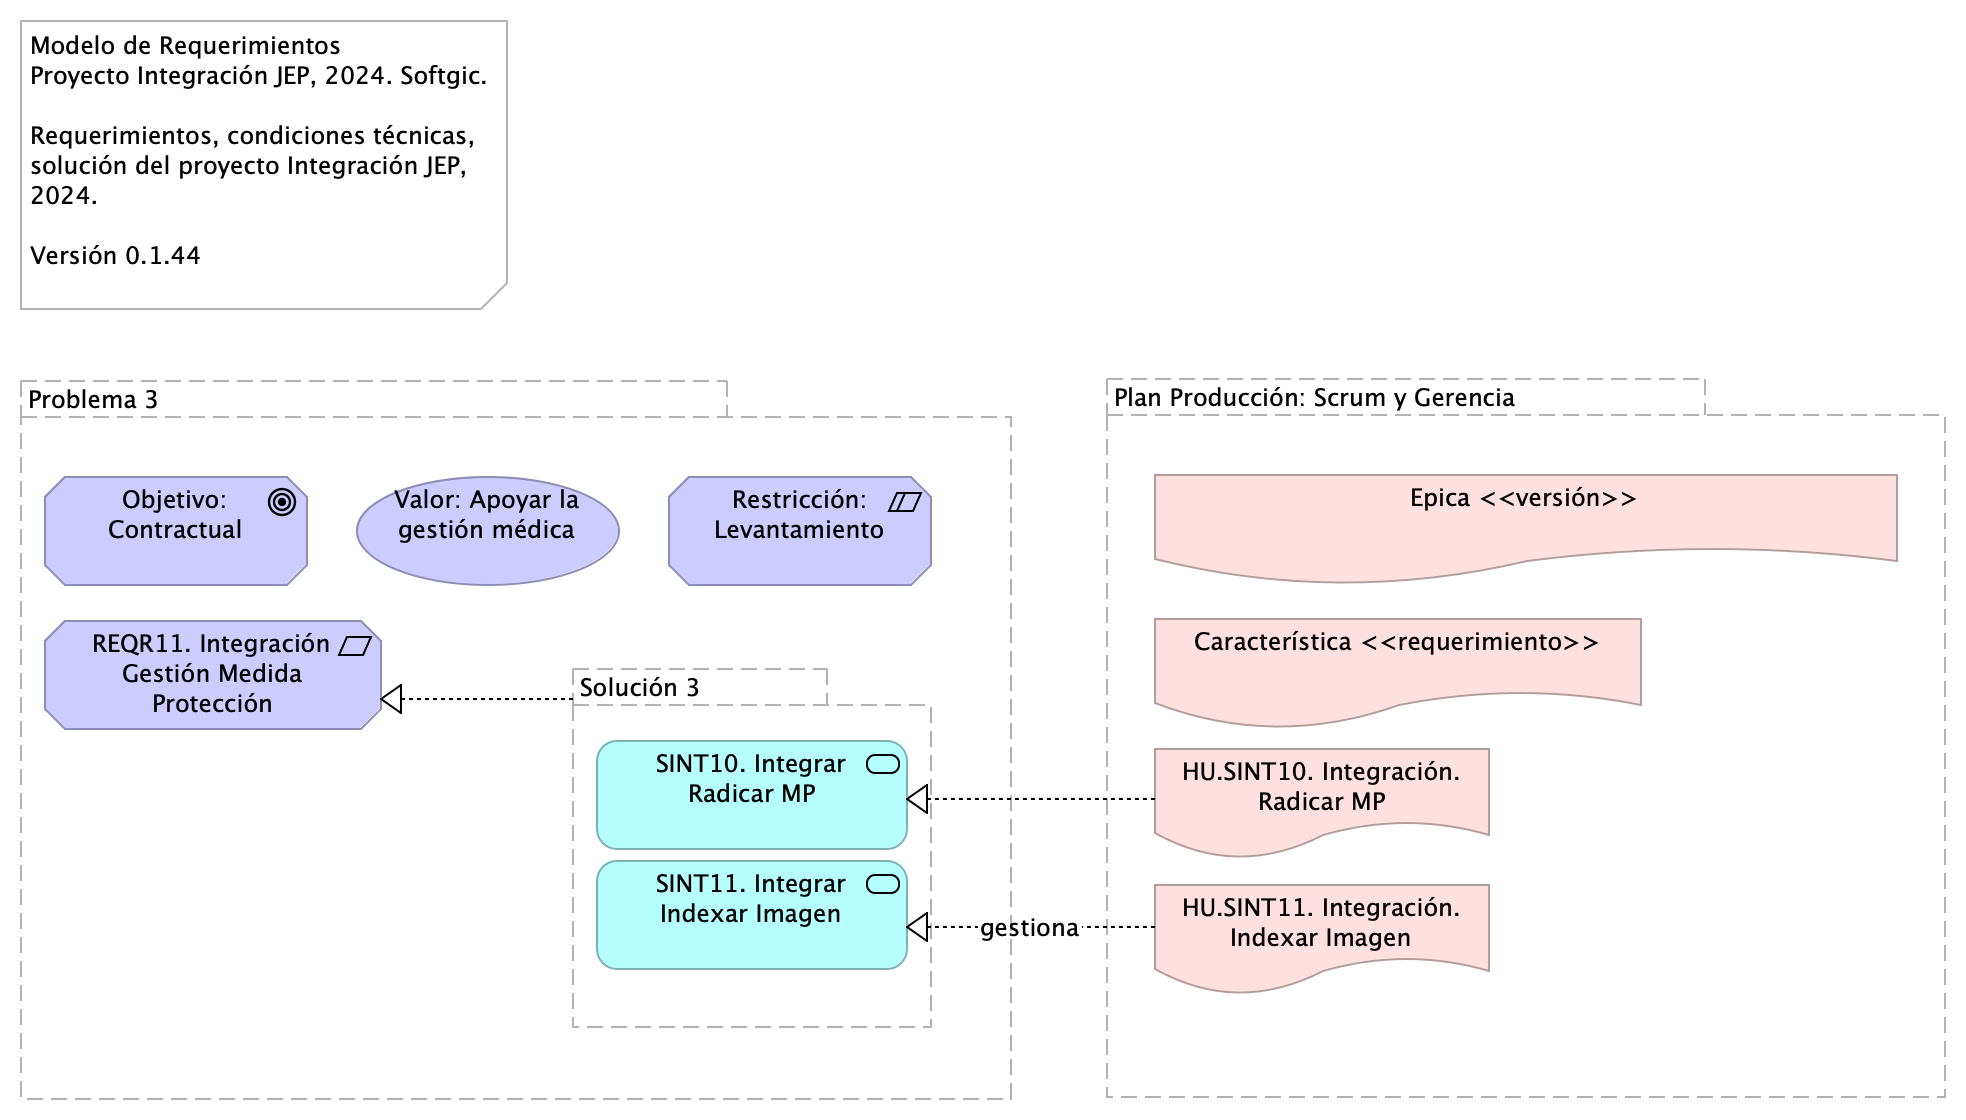
\includegraphics[width=\textwidth,height=5.20833in]{images/05.REQR.1n.1b.RequerimientoREQR11.png}
\caption{05.REQR.1n.1b. Requerimiento REQR11. \emph{Fuente: Repositorio
arquitectura Integración JEP
(2024)}}\label{fig:id-8b4c8be23da34d399e8127a08a5204b8}
\end{figure}

\subsubsection{Plan Producción: Scrum y
Gerencia}\label{sec:plan-producciuxf3n-scrum-y-gerencia}

\subsubsection{Problema 3}\label{sec:problema-3}

\subsubsection{Objetivo: Contractual}\label{sec:objetivo-contractual}

El requerimiento tiene carácter contractual.

\subsubsection{Valor: Apoyar la gestión medida
protección}\label{sec:valor-apoyar-la-gestiuxf3n-medida-protecciuxf3n}

El requerimientos genera entregables de valor para la gestión de medida
de protección JEP.

\subsubsection{Restricción:
Levantamiento}\label{sec:restricciuxf3n-levantamiento}

El requerimiento está condicionado por la completitud del levantamiento.

\subsubsection{REQR11. Integración Gestión Medida
Protección}\label{sec:reqr11.-integraciuxf3n-gestiuxf3n-medida-protecciuxf3n}

Atendiendo la necesidad de (\ldots) se requiere integrar la gestión
médica JEP, como exposición de las capacidades Radicar MP y Indexar
Imagen, las cuales se encuentran en (\ldots).

Fuente: gestionMedidaProteccion (pdf).

\subsubsection{Índice de la documentación (casos de
uso)}\label{sec:uxedndice-de-la-documentaciuxf3n-casos-de-uso}

\begin{enumerate}
\def\labelenumi{\arabic{enumi}.}
\tightlist
\item
  Caso de Uso 1. Integrar Radicar MP
\item
  Caso de Uso 2. Integrar Indexar Imagen
\end{enumerate}

Los casos de uso se detallan en anexo más adelante.

\subsubsection{Solución 3}\label{sec:soluciuxf3n-3}

\subsubsection{SINT10. Integrar Radicar
MP}\label{sec:sint10.-integrar-radicar-mp}

Tareas de desarrollo

\begin{itemize}
\tightlist
\item
  Interoperabilidad IOP1. Transporte / Entrega Consulta Negocio
\item
  Modelo de datos (XML, RBDMS, \ldots)
\item
  Esquema de datos (XSD, DTD, JSON-E\ldots)
\item
  Contratos de interoperabilidad (WSDL, API\ldots)
\item
  Mensajes petición IN (API, XML\ldots)
\item
  Mensajes respuesta OUT (API, XML\ldots)
\item
  Mensajes excepción (API, XML\ldots)
\item
  Transporte (REST, SOAP)
\item
  Función lógica (JEE, \ldots)
\item
  Registro y envío de actividad
\end{itemize}

\subsubsection{SINT11. Integrar Indexar
Imagen}\label{sec:sint11.-integrar-indexar-imagen}

Tareas de desarrollo

\begin{itemize}
\tightlist
\item
  Interoperabilidad IOP1. Transporte / Entrega Consulta Negocio
\item
  Modelo de datos (XML, RBDMS, \ldots)
\item
  Esquema de datos (XSD, DTD, JSON-E\ldots)
\item
  Contratos de interoperabilidad (WSDL, API\ldots)
\item
  Mensajes petición IN (API, XML\ldots)
\item
  Mensajes respuesta OUT (API, XML\ldots)
\item
  Mensajes excepción (API, XML\ldots)
\item
  Transporte (REST, SOAP)
\item
  Función lógica (JEE, \ldots)
\item
  Registro y envío de actividad
\end{itemize}

\subsection{Especificación CU Requerimiento
REQR11}\label{sec:especificaciuxf3n-cu-requerimiento-reqr11}

\begin{quote}
Casos de Uso Proyecto Integración JEP, 2024. Softgic. Especificaciones
de integraciones (CU), condiciones de interoperabilidad, pruebas
técnicas, entregables. Versión 0.1.97
\end{quote}

Documentación de los casos de uso de integración del proyecto JEP
relacionados con los requerimientos. COndiciones de interoperabilidad,
pruebas técnicas y entregables.

Fuente: Acta de requerimientos Integración Plani - Proceso
Precontractual\_V4.pdf

\begin{figure}
\centering
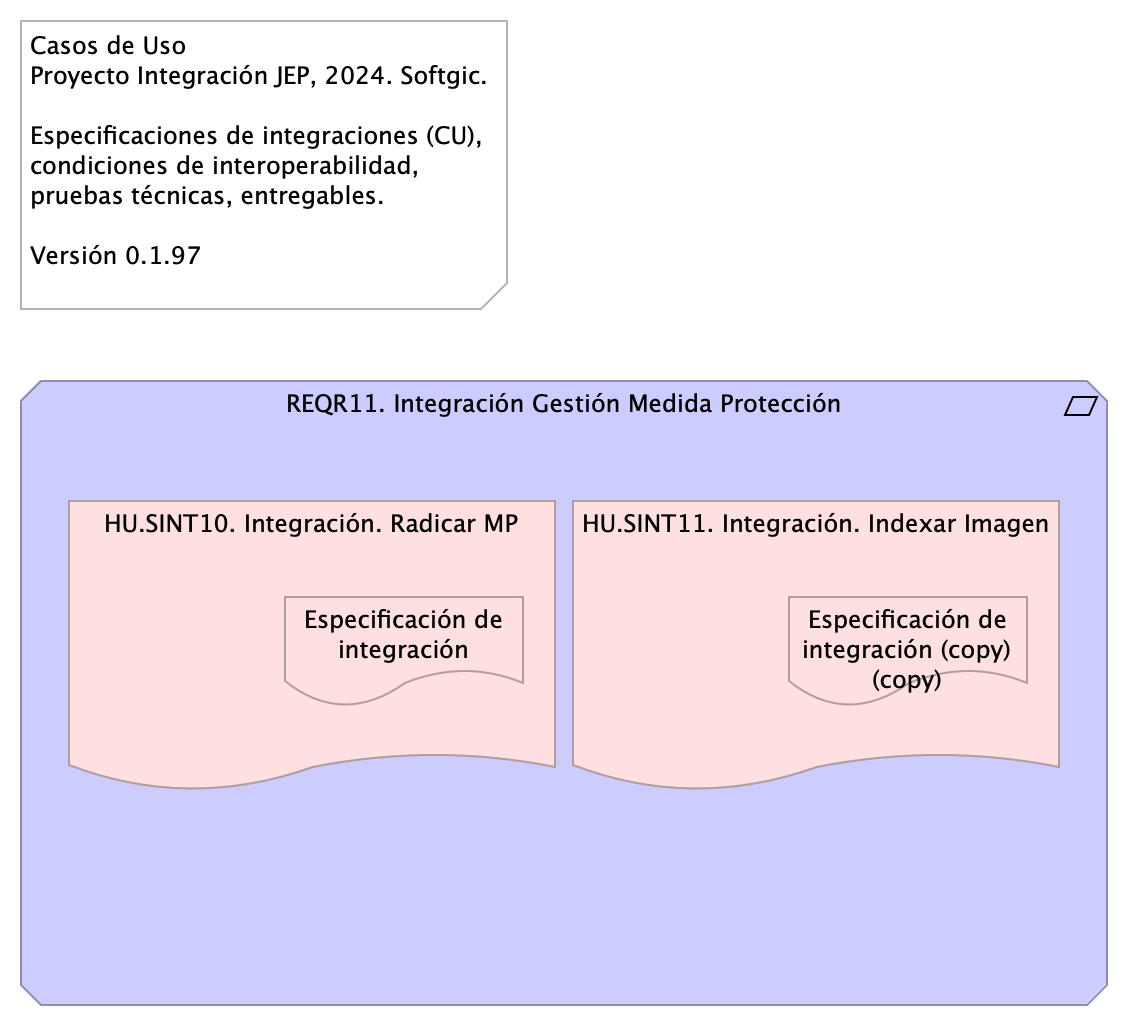
\includegraphics[width=\textwidth,height=5.20833in]{images/05.REQR.2n.4n.CasosdeUsoREQR11.png}
\caption{05.REQR.2n.4n. Casos de Uso REQR11. \emph{Fuente: Repositorio
arquitectura Integración JEP
(2024)}}\label{fig:id-086d2945e90743568dc1ce48079c40bf}
\end{figure}

\subsubsection{REQR11. Integración Gestión Medida
Protección}\label{sec:reqr11.-integraciuxf3n-gestiuxf3n-medida-protecciuxf3n-1}

Atendiendo la necesidad de (\ldots) se requiere integrar la gestión
médica JEP, como exposición de las capacidades Radicar MP y Indexar
Imagen, las cuales se encuentran en (\ldots).

Fuente: gestionMedidaProteccion (pdf).

\subsubsection{Índice de la documentación (casos de
uso)}\label{sec:uxedndice-de-la-documentaciuxf3n-casos-de-uso-1}

\begin{enumerate}
\def\labelenumi{\arabic{enumi}.}
\tightlist
\item
  Caso de Uso 1. Integrar Radicar MP
\item
  Caso de Uso 2. Integrar Indexar Imagen
\end{enumerate}

Los casos de uso se detallan en anexo más adelante.

\subsubsection{HU.SINT10. Integración. Radicar
MP}\label{sec:hu.sint10.-integraciuxf3n.-radicar-mp}

\subsubsection{Especificación de
integración}\label{sec:especificaciuxf3n-de-integraciuxf3n}

Radicar MP. Esta integración permite radicar una solicitud de medida de
protección.

Detalles:

\begin{itemize}
\tightlist
\item
  Dominio/mercurio/gestionMedidaProteccion/radicarMP Method: POST
\item
  Content-Type: application/json.
\end{itemize}

Ver fuente anexo técnico: gestionMedidaProteccion (pdf).

\paragraph{Elementos}\label{sec:elementos}

Elegir y describir los elementos de la actual integración.

\begin{itemize}
\tightlist
\item[$\boxtimes$]
  App consumidora (A)
\item[$\boxtimes$]
  Mensaje
\item[$\square$]
  Canal
\item[$\square$]
  Ruteo
\item[$\square$]
  Traducción
\item[$\boxtimes$]
  App proveedora (B)
\item[$\square$]
  Monitoreo
\end{itemize}

Aplicación consumidora A: Aplicación JEP. Aplicación proveedora B: MP

Mensaje solicitud: (ver estándar de nombramiento) Radicar MP.

\begin{itemize}
\tightlist
\item
  Tipo: TXT \textbar{} SOAP \textbar{} XML \textbar{} JSN \textbar{} YML
  \textbar{} BASE64
\item
  Contenido: Usuario o identidad Conti
\end{itemize}

Mensaje respuesta: Rpta. Ingreso a Conti

\begin{itemize}
\tightlist
\item
  Tipo: TXT \textbar{} SOAP \textbar{} XML \textbar{} JSN \textbar{} YML
  \textbar{} BASE64
\item
  Contenido: Estado de solicitud de ingreso a Conti
\end{itemize}

Mensaje excepción: Rpta. Ingreso a Conti

\begin{itemize}
\tightlist
\item
  Tipo: TXT \textbar{} SOAP \textbar{} XML \textbar{} JSN \textbar{} YML
  \textbar{} BASE64
\item
  Contenido: Código de respuesta: HTTP 500 \textbar{} TXT \textbar{}
  Numeración (entero)
\end{itemize}

\paragraph{Diseño}\label{sec:diseuxf1o}

Message Construct \textbar{} Message Routing \textbar{} Message
Transformation \textbar{} Messaging Endpoints \textbar{} Messaging
Channels \textbar{} \ldots{}

La aplicación consumidora y proveedora compartirán capacidades mediante
un mensaje de autenticación (Message Construct).

\paragraph{Matriz de
interoperabilidad}\label{sec:matriz-de-interoperabilidad}

Detalle del intercambio entre sistemas de información o aplicaciones.

App Plani requiere compartir Información {[}I{]}, Funcionalidad {[}F{]},
Seguridad o Servicios {[}S{]} con la App Plani.

\begin{longtable}[]{@{}llllll@{}}
\caption{Matriz de interoperabilidad del CU Radicar MP.}\tabularnewline
\toprule\noalign{}
& MP & App & Legali & Plani & Otros \\
\midrule\noalign{}
\endfirsthead
\toprule\noalign{}
& MP & App & Legali & Plani & Otros \\
\midrule\noalign{}
\endhead
\bottomrule\noalign{}
\endlastfoot
App (A) & F & & & & \\
MP (B) & & F & & & \\
Legali & & & & & \\
Otros Sistemas & & & & & \\
\end{longtable}

\paragraph{Pruebas Realizables}\label{sec:pruebas-realizables}

Por cada caso de prueba de integración describir el resultado del
intercambio entre sistemas de información o aplicaciones según la Matriz
de interoperabilidad.

\begin{itemize}
\tightlist
\item
  PRUB1. Consumo radicar.
\item
  PRUB2. Falla consumo radicar.
\end{itemize}

\subsubsection{HU.SINT11. Integración. Indexar
Imagen}\label{sec:hu.sint11.-integraciuxf3n.-indexar-imagen}

\subsubsection{Especificación de
integración}\label{sec:especificaciuxf3n-de-integraciuxf3n-1}

Indexar Imagen. Esta integración permite agregar nuevos archivos a la
medida de Protección.

Detalles:

\begin{itemize}
\tightlist
\item
  Dominio/mercurio/gestionMedidaProteccion/IndexarImagen Method: POST
\item
  Content-Type: application/json
\end{itemize}

Ver fuente anexo técnico: gestionMedidaProteccion (pdf).

\paragraph{Elementos}\label{sec:elementos-1}

Elegir y describir los elementos de la actual integración.

\begin{itemize}
\tightlist
\item[$\boxtimes$]
  App consumidora (A)
\item[$\boxtimes$]
  Mensaje
\item[$\square$]
  Canal
\item[$\square$]
  Ruteo
\item[$\square$]
  Traducción
\item[$\boxtimes$]
  App proveedora (B)
\item[$\square$]
  Monitoreo
\end{itemize}

Aplicación consumidora A: Aplicación JEP. Aplicación proveedora B: MP

Mensaje solicitud: (ver estándar de nombramiento) Radicar MP.

\begin{itemize}
\tightlist
\item
  Tipo: TXT \textbar{} SOAP \textbar{} XML \textbar{} JSN \textbar{} YML
  \textbar{} BASE64
\item
  Contenido: Usuario o identidad Conti
\end{itemize}

Mensaje respuesta: Rpta. Ingreso a Conti

\begin{itemize}
\tightlist
\item
  Tipo: TXT \textbar{} SOAP \textbar{} XML \textbar{} JSN \textbar{} YML
  \textbar{} BASE64
\item
  Contenido: Estado de solicitud de ingreso a Conti
\end{itemize}

Mensaje excepción: Rpta. Ingreso a Conti

\begin{itemize}
\tightlist
\item
  Tipo: TXT \textbar{} SOAP \textbar{} XML \textbar{} JSN \textbar{} YML
  \textbar{} BASE64
\item
  Contenido: Código de respuesta: HTTP 500 \textbar{} TXT \textbar{}
  Numeración (entero)
\end{itemize}

\paragraph{Diseño}\label{sec:diseuxf1o-1}

Message Construct \textbar{} Message Routing \textbar{} Message
Transformation \textbar{} Messaging Endpoints \textbar{} Messaging
Channels \textbar{} \ldots{}

La aplicación consumidora y proveedora compartirán capacidades mediante
un mensaje de autenticación (Message Construct).

\paragraph{Matriz de
interoperabilidad}\label{sec:matriz-de-interoperabilidad-1}

Detalle del intercambio entre sistemas de información o aplicaciones.

App Plani requiere compartir Información {[}I{]}, Funcionalidad {[}F{]},
Seguridad o Servicios {[}S{]} con la App Plani.

\begin{longtable}[]{@{}llllll@{}}
\caption{Matriz de interoperabilidad del CU Indexar
Imagen.}\tabularnewline
\toprule\noalign{}
& MP & App & Legali & Plani & Otros \\
\midrule\noalign{}
\endfirsthead
\toprule\noalign{}
& MP & App & Legali & Plani & Otros \\
\midrule\noalign{}
\endhead
\bottomrule\noalign{}
\endlastfoot
App (A) & F & & & & \\
MP (B) & & F & & & \\
Legali & & & & & \\
Otros Sistemas & & & & & \\
\end{longtable}

\paragraph{Pruebas Realizables}\label{sec:pruebas-realizables-1}

Por cada caso de prueba de integración describir el resultado del
intercambio entre sistemas de información o aplicaciones según la Matriz
de interoperabilidad.

\begin{itemize}
\tightlist
\item
  PRUB1. Consumo indexar.
\item
  PRUB2. Falla consumo indexar.
\end{itemize}

\subsection{Requerimiento Integración envío de peticiones LEGALi x CONTi
(REQR13)}\label{sec:requerimiento-integraciuxf3n-envuxedo-de-peticiones-legali-x-conti-reqr13}

\begin{quote}
Modelo de Requerimientos Proyecto Integración JEP, 2024. Softgic.
Requerimientos, condiciones técnicas, solución del proyecto Integración
JEP, 2024. Versión 0.1.39
\end{quote}

Del alcance del proyecto,

\begin{enumerate}
\def\labelenumi{\arabic{enumi}.}
\tightlist
\item
  Implementación de 20 o más servicios de integración al 31 de diciembre
  del 2024.
\item
  Soporte solución de integración a julio 2025.
\end{enumerate}

Establecemos las bases para el modelo de requerimientos de esta
solución, el cual limita la demanda a:

\begin{itemize}
\tightlist
\item
  Desarrollar únicamente nuevos servicios de integración con el patrón
  de integración empresarial (ESB, Camel K de Apache) propuesto en el
  modelo de interoperabilidad de esta solución.
\item
  Implementar en esta solución de integración las condiciones
  tecnológicas JEP, entendidas como requerimientos no funcionales de
  arquitectura, presentes en el Anexo Nro. 1.1 -- Anexo técnico
  evolución plataforma de interoperabilidad -- Ficha Técnica.
\item
  No son requerimientos de este proyecto el implementar otro tipos de
  requerimientos no expresados aquí, como por ejemplo, migrar los
  servicios existentes de modelo integración directa (EIA) esta solución
  de integración empresarial, o implementar soluciones en las
  aplicaciones de software de la JEP.
\end{itemize}

Para la implementación de los ítems relacionados en el Anexo Nro. 1.1 --
Anexo técnico evolución plataforma de interoperabilidad -- Ficha Técnica
la hoja ``Categorías de Cotización'' contiene las necesidades a
contratar en el ámbito de la evolución tecnológica del modelo de
interoperabilidad y los desarrollos de interoperabilidad tanto con
sistemas internos, como con entidades externas. En la hoja ``Estándares
Desarrollo y Producto'' del archivo mencionado se indican los estándares
recomendados por el fabricante, para tener en cuenta en la entrega de
los servicios que se cotizan.

El Anexo Nro. 1.2 -- Acuerdos de Niveles de Servicio, explica el
procedimiento con el que se dará atención a consultas o solución de
incidencias, tanto en los sistemas operativos, como en los servicios de
interoperabilidad existentes en la actualidad y aquellos que se
contratarán en este proceso, en el sistema Bus de Interoperabilidad
implementado en la Jurisdicción Especial para la Paz.

Fuente: Justificativo de la Contratación Invitación Pública.

\begin{figure}
\centering
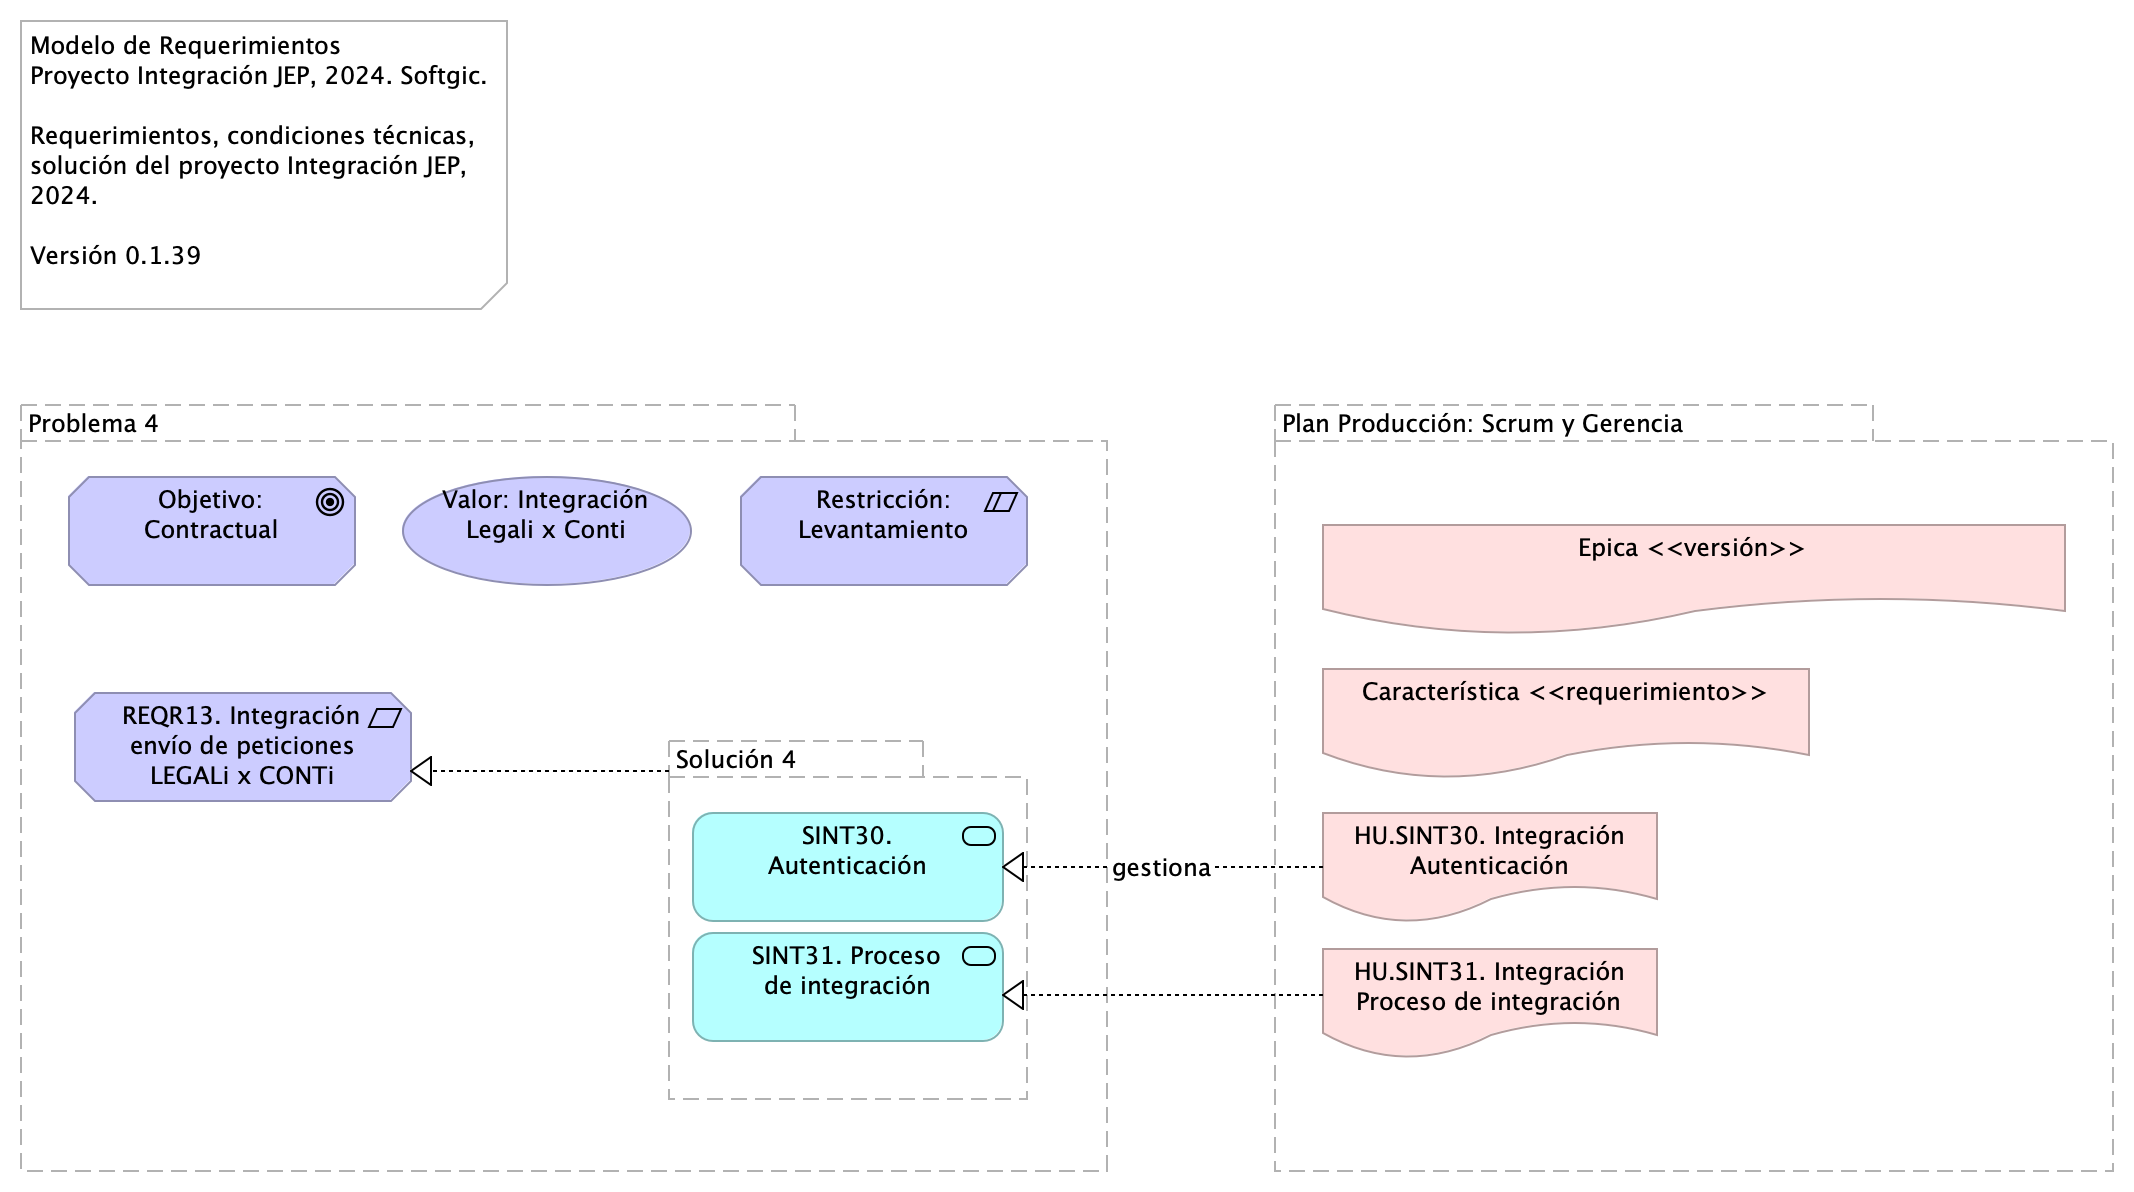
\includegraphics[width=\textwidth,height=5.20833in]{images/05.REQR.1n.1d.RequerimientoREQR13.png}
\caption{05.REQR.1n.1d. Requerimiento REQR13. \emph{Fuente: Repositorio
arquitectura Integración JEP
(2024)}}\label{fig:id-c16e7b2e768c4de7ab50fb13972e5c08}
\end{figure}

\subsubsection{Problema 4}\label{sec:problema-4}

\subsubsection{Objetivo: Contractual}\label{sec:objetivo-contractual-1}

El requerimiento tiene carácter contractual.

\subsubsection{Valor: Integración Legali x
Conti}\label{sec:valor-integraciuxf3n-legali-x-conti}

Integración del gestor documental con el gestor de casos Legali.

\subsubsection{Restricción:
Levantamiento}\label{sec:restricciuxf3n-levantamiento-1}

El requerimiento está condicionado por la completitud del levantamiento.

\subsubsection{REQR13. Integración envío de peticiones LEGALi x
CONTi}\label{sec:reqr13.-integraciuxf3n-envuxedo-de-peticiones-legali-x-conti}

Atendiendo la necesidad de Justicia Digital, se requiere implementar la
integración de Legali como la exposición de las capacidades
\emph{Autenticación y Procesos de integración}.

Fuente: Servicio de integración LEGALi - Envío de peticiones - v5 (pdf).
José Carlos Schröder Júnior.

\subsubsection{Índice de la documentación (casos de
uso)}\label{sec:uxedndice-de-la-documentaciuxf3n-casos-de-uso-2}

\begin{enumerate}
\def\labelenumi{\arabic{enumi}.}
\tightlist
\item
  Caso de Uso 1. Integrar Autenticación
\item
  Caso de Uso 2. Integrar Procesos de integración
\end{enumerate}

Los casos de uso se detallan en anexo más adelante.

\subsubsection{Solución 4}\label{sec:soluciuxf3n-4}

\subsubsection{SINT30.
Autenticación}\label{sec:sint30.-autenticaciuxf3n}

Tareas de desarrollo

\begin{itemize}
\tightlist
\item
  Interoperabilidad IOP1. Transporte / Entrega Consulta Negocio\\
\item
  Modelo de datos (XML, RBDMS, \ldots)
\item
  Esquema de datos (XSD, DTD, JSON-E\ldots)
\item
  Contratos de interoperabilidad (WSDL, API\ldots)
\item
  Mensajes petición IN (API, XML\ldots)
\item
  Mensajes respuesta OUT (API, XML\ldots)
\item
  Mensajes excepción (API, XML\ldots)
\item
  Transporte (REST, SOAP)
\item
  Función lógica (JEE, \ldots)
\item
  Registro y envío de actividad
\end{itemize}

\subsubsection{SINT31. Proceso de
integración}\label{sec:sint31.-proceso-de-integraciuxf3n}

Tareas de desarrollo

\begin{itemize}
\tightlist
\item
  Interoperabilidad IOP1. Transporte / Entrega Consulta Negocio\\
\item
  Modelo de datos (XML, RBDMS, \ldots)
\item
  Esquema de datos (XSD, DTD, JSON-E\ldots)
\item
  Contratos de interoperabilidad (WSDL, API\ldots)
\item
  Mensajes petición IN (API, XML\ldots)
\item
  Mensajes respuesta OUT (API, XML\ldots)
\item
  Mensajes excepción (API, XML\ldots)
\item
  Transporte (REST, SOAP)
\item
  Función lógica (JEE, \ldots)
\item
  Registro y envío de actividad
\end{itemize}

\subsubsection{Plan Producción: Scrum y
Gerencia}\label{sec:plan-producciuxf3n-scrum-y-gerencia-1}

\subsection{Especificación CU Requerimiento
REQR13}\label{sec:especificaciuxf3n-cu-requerimiento-reqr13}

\begin{quote}
Casos de Uso Proyecto Integración JEP, 2024. Softgic. Especificaciones
de integraciones (CU), condiciones de interoperabilidad, pruebas
técnicas, entregables. Versión 0.1.98
\end{quote}

Documentación de los casos de uso de integración del proyecto JEP
relacionados con los requerimientos. COndiciones de interoperabilidad,
pruebas técnicas y entregables.

Fuente: Acta de requerimientos Integración Plani - Proceso
Precontractual\_V4.pdf

\begin{figure}
\centering
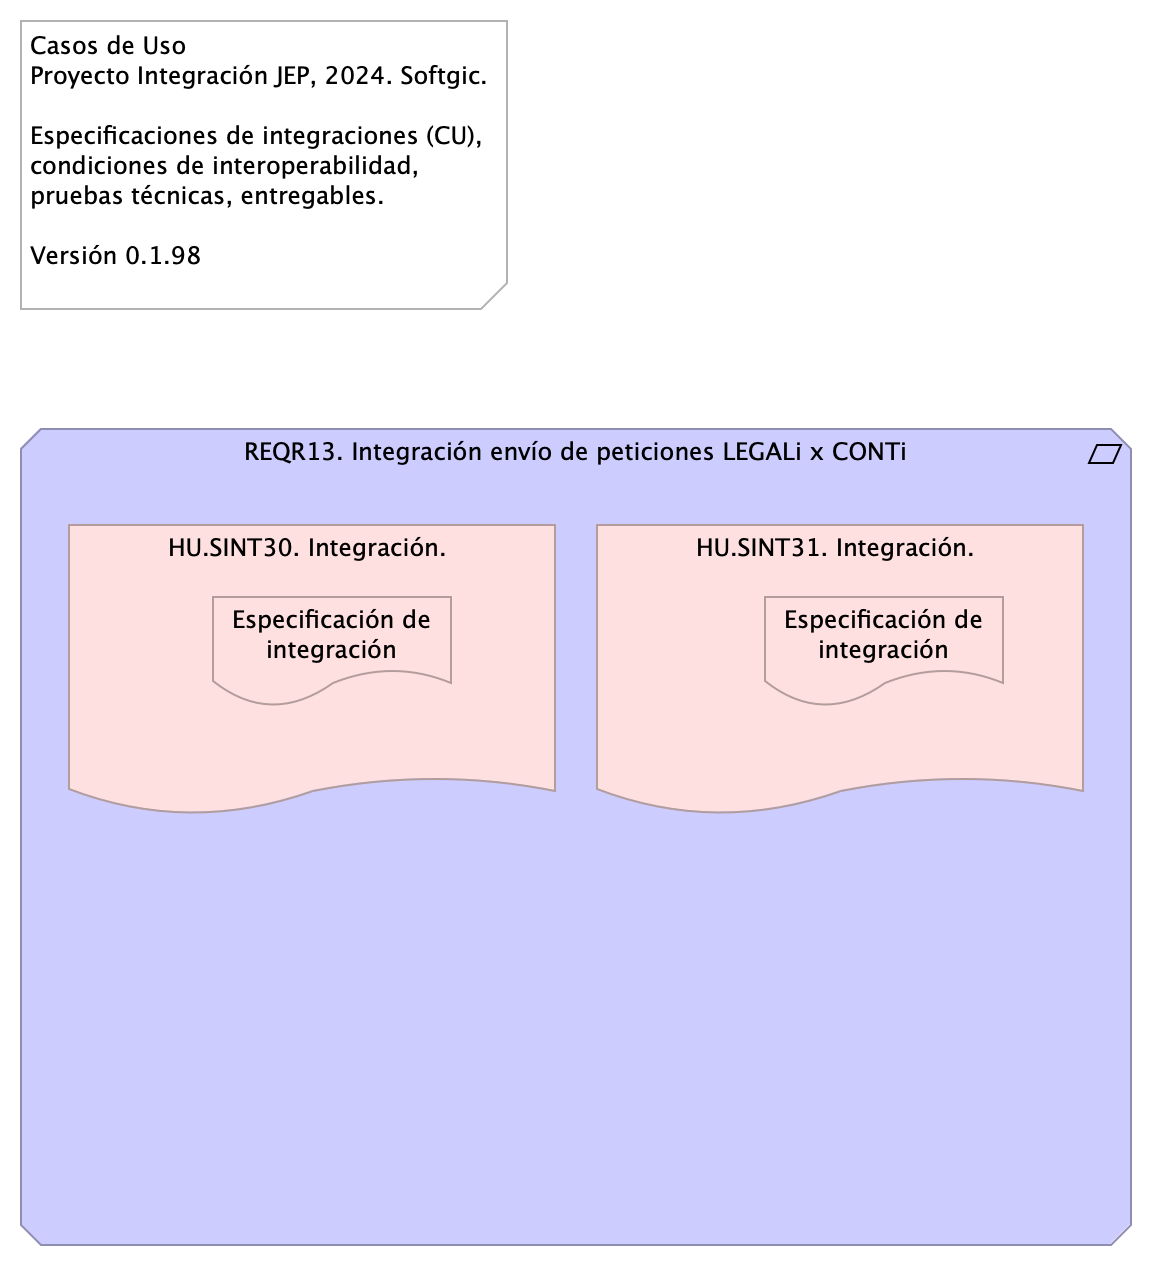
\includegraphics[width=\textwidth,height=5.20833in]{images/05.REQR.2n.5n.CasosdeUsoREQR13.png}
\caption{05.REQR.2n.5n. Casos de Uso REQR13. \emph{Fuente: Repositorio
arquitectura Integración JEP
(2024)}}\label{fig:id-d6e0a0d4192e4eb6955c7363e93a0bf5}
\end{figure}

\subsubsection{REQR13. Integración envío de peticiones LEGALi x
CONTi}\label{sec:reqr13.-integraciuxf3n-envuxedo-de-peticiones-legali-x-conti-1}

Atendiendo la necesidad de Justicia Digital, se requiere implementar la
integración de Legali como la exposición de las capacidades
\emph{Autenticación y Procesos de integración}.

Fuente: Servicio de integración LEGALi - Envío de peticiones - v5 (pdf).
José Carlos Schröder Júnior.

\subsubsection{Índice de la documentación (casos de
uso)}\label{sec:uxedndice-de-la-documentaciuxf3n-casos-de-uso-3}

\begin{enumerate}
\def\labelenumi{\arabic{enumi}.}
\tightlist
\item
  Caso de Uso 1. Integrar Autenticación
\item
  Caso de Uso 2. Integrar Procesos de integración
\end{enumerate}

Los casos de uso se detallan en anexo más adelante.

\subsubsection{HU.SINT30.
Integración.}\label{sec:hu.sint30.-integraciuxf3n.}

\subsubsection{Especificación de
integración}\label{sec:especificaciuxf3n-de-integraciuxf3n-2}

Solicitar autenticación a la aplicación Conti y devolver resultado de la
solicitud de ingreso a la aplicación Plani.

\paragraph{Elementos}\label{sec:elementos-2}

Elegir y describir los elementos de la actual integración.

\begin{itemize}
\tightlist
\item[$\boxtimes$]
  App consumidora (A)
\item[$\boxtimes$]
  Mensaje
\item[$\square$]
  Canal
\item[$\square$]
  Ruteo
\item[$\square$]
  Traducción
\item[$\boxtimes$]
  App proveedora (B)
\item[$\square$]
  Monitoreo
\end{itemize}

Aplicación consumidora A: Plani. Aplicación proveedora B: Conti

Mensaje solicitud: (ver estándar de nombramiento) Ingreso a Conti

\begin{itemize}
\tightlist
\item
  Tipo: TXT \textbar{} SOAP \textbar{} XML \textbar{} JSN \textbar{} YML
  \textbar{} BASE64
\item
  Contenido: Usuario o identidad Conti
\end{itemize}

Mensaje respuesta: Rpta. Ingreso a Conti

\begin{itemize}
\tightlist
\item
  Tipo: TXT \textbar{} SOAP \textbar{} XML \textbar{} JSN \textbar{} YML
  \textbar{} BASE64
\item
  Contenido: Estado de solicitud de ingreso a Conti
\end{itemize}

Mensaje excepción: Rpta. Ingreso a Conti

\begin{itemize}
\tightlist
\item
  Tipo: TXT \textbar{} SOAP \textbar{} XML \textbar{} JSN \textbar{} YML
  \textbar{} BASE64
\item
  Contenido: Código de respuesta: HTTP 500 \textbar{} TXT \textbar{}
  Numeración (entero)
\end{itemize}

\paragraph{Diseño}\label{sec:diseuxf1o-2}

Message Construct \textbar{} Message Routing \textbar{} Message
Transformation \textbar{} Messaging Endpoints \textbar{} Messaging
Channels \textbar{} \ldots{}

La aplicación consumidora y proveedora compartirán capacidades mediante
un mensaje de autenticación (Message Construct).

\paragraph{Matriz de
interoperabilidad}\label{sec:matriz-de-interoperabilidad-2}

Detalle del intercambio entre sistemas de información o aplicaciones.

App Plani requiere compartir Información {[}I{]}, Funcionalidad {[}F{]},
Seguridad o Servicios {[}S{]} con la App Plani.

\begin{longtable}[]{@{}lllll@{}}
\caption{Matriz de interoperabilidad del CU Ingreso a
Conti.}\tabularnewline
\toprule\noalign{}
& Conti & Plani & Legali & Otros \\
\midrule\noalign{}
\endfirsthead
\toprule\noalign{}
& Conti & Plani & Legali & Otros \\
\midrule\noalign{}
\endhead
\bottomrule\noalign{}
\endlastfoot
Conti (B) & X & Seguridad & & \\
Plani (A) & & X & & \\
Legali & & & X & \\
Otros Sistemas & & & & X \\
\end{longtable}

\paragraph{Pruebas Realizables}\label{sec:pruebas-realizables-2}

Por cada caso de prueba de integración describir el resultado del
intercambio entre sistemas de información o aplicaciones según la Matriz
de interoperabilidad.

\begin{itemize}
\tightlist
\item
  PRUB1. Consumo: la aplicación consumidora Plani no recibe una
  respuesta a tiempo.
\item
  PRUB2. Ingreso: la aplicación proveedora Conti no provee un ingreso
  autorizado.
\end{itemize}

\subsubsection{HU.SINT31.
Integración.}\label{sec:hu.sint31.-integraciuxf3n.}

\subsubsection{Especificación de
integración}\label{sec:especificaciuxf3n-de-integraciuxf3n-3}

Radicar MP. Esta integración permite radicar una solicitud de medida de
protección.

Detalles:

\begin{itemize}
\tightlist
\item
  Dominio/mercurio/gestionMedidaProteccion/radicarMP Method: POST
\item
  Content-Type: application/json.
\end{itemize}

Ver fuente anexo técnico: gestionMedidaProteccion (pdf).

\paragraph{Elementos}\label{sec:elementos-3}

Elegir y describir los elementos de la actual integración.

\begin{itemize}
\tightlist
\item[$\boxtimes$]
  App consumidora (A)
\item[$\boxtimes$]
  Mensaje
\item[$\square$]
  Canal
\item[$\square$]
  Ruteo
\item[$\square$]
  Traducción
\item[$\boxtimes$]
  App proveedora (B)
\item[$\square$]
  Monitoreo
\end{itemize}

Aplicación consumidora A: Aplicación JEP. Aplicación proveedora B: MP

Mensaje solicitud: (ver estándar de nombramiento) Radicar MP.

\begin{itemize}
\tightlist
\item
  Tipo: TXT \textbar{} SOAP \textbar{} XML \textbar{} JSN \textbar{} YML
  \textbar{} BASE64
\item
  Contenido: Usuario o identidad Conti
\end{itemize}

Mensaje respuesta: Rpta. Ingreso a Conti

\begin{itemize}
\tightlist
\item
  Tipo: TXT \textbar{} SOAP \textbar{} XML \textbar{} JSN \textbar{} YML
  \textbar{} BASE64
\item
  Contenido: Estado de solicitud de ingreso a Conti
\end{itemize}

Mensaje excepción: Rpta. Ingreso a Conti

\begin{itemize}
\tightlist
\item
  Tipo: TXT \textbar{} SOAP \textbar{} XML \textbar{} JSN \textbar{} YML
  \textbar{} BASE64
\item
  Contenido: Código de respuesta: HTTP 500 \textbar{} TXT \textbar{}
  Numeración (entero)
\end{itemize}

\paragraph{Diseño}\label{sec:diseuxf1o-3}

Message Construct \textbar{} Message Routing \textbar{} Message
Transformation \textbar{} Messaging Endpoints \textbar{} Messaging
Channels \textbar{} \ldots{}

La aplicación consumidora y proveedora compartirán capacidades mediante
un mensaje de autenticación (Message Construct).

\paragraph{Matriz de
interoperabilidad}\label{sec:matriz-de-interoperabilidad-3}

Detalle del intercambio entre sistemas de información o aplicaciones.

App Plani requiere compartir Información {[}I{]}, Funcionalidad {[}F{]},
Seguridad o Servicios {[}S{]} con la App Plani.

\begin{longtable}[]{@{}llllll@{}}
\caption{Matriz de interoperabilidad del CU Radicar MP.}\tabularnewline
\toprule\noalign{}
& MP & App & Legali & Plani & Otros \\
\midrule\noalign{}
\endfirsthead
\toprule\noalign{}
& MP & App & Legali & Plani & Otros \\
\midrule\noalign{}
\endhead
\bottomrule\noalign{}
\endlastfoot
App (A) & F & & & & \\
MP (B) & & F & & & \\
Legali & & & & & \\
Otros Sistemas & & & & & \\
\end{longtable}

\paragraph{Pruebas Realizables}\label{sec:pruebas-realizables-3}

Por cada caso de prueba de integración describir el resultado del
intercambio entre sistemas de información o aplicaciones según la Matriz
de interoperabilidad.

\begin{itemize}
\tightlist
\item
  PRUB1. Consumo radicar.
\item
  PRUB2. Falla consumo radicar.
\end{itemize}

\newpage

\section{Modelo de Despliegue de Requerimientos de Interoperabilidad
Proyecto
JEP}\label{sec:modelo-de-despliegue-de-requerimientos-de-interoperabilidad-proyecto-jep}

\subsection{Despliegue de Entrega del
Requerimiento}\label{sec:despliegue-de-entrega-del-requerimiento}

\begin{quote}
Integraciones JEP, 2024 Integración JEP. Softgic. Plan de Entregas del
proyecto de integración y despliegue JEP, iteraciones y Entregables por
versión. versión 0.1.18
\end{quote}

Los servicios implementados contenidos en los requerimientos se pueden
desplegar sobre la red de unidades de despliegue (pods) dispuesta por la
JEP y acordada con el contratista.

En esta organización propuesta, los servicios de integración
implementados pueden ser desplegados en uno, o varios contenedores, y en
unidades de despliegue (pods) distintas.

\begin{figure}
\centering
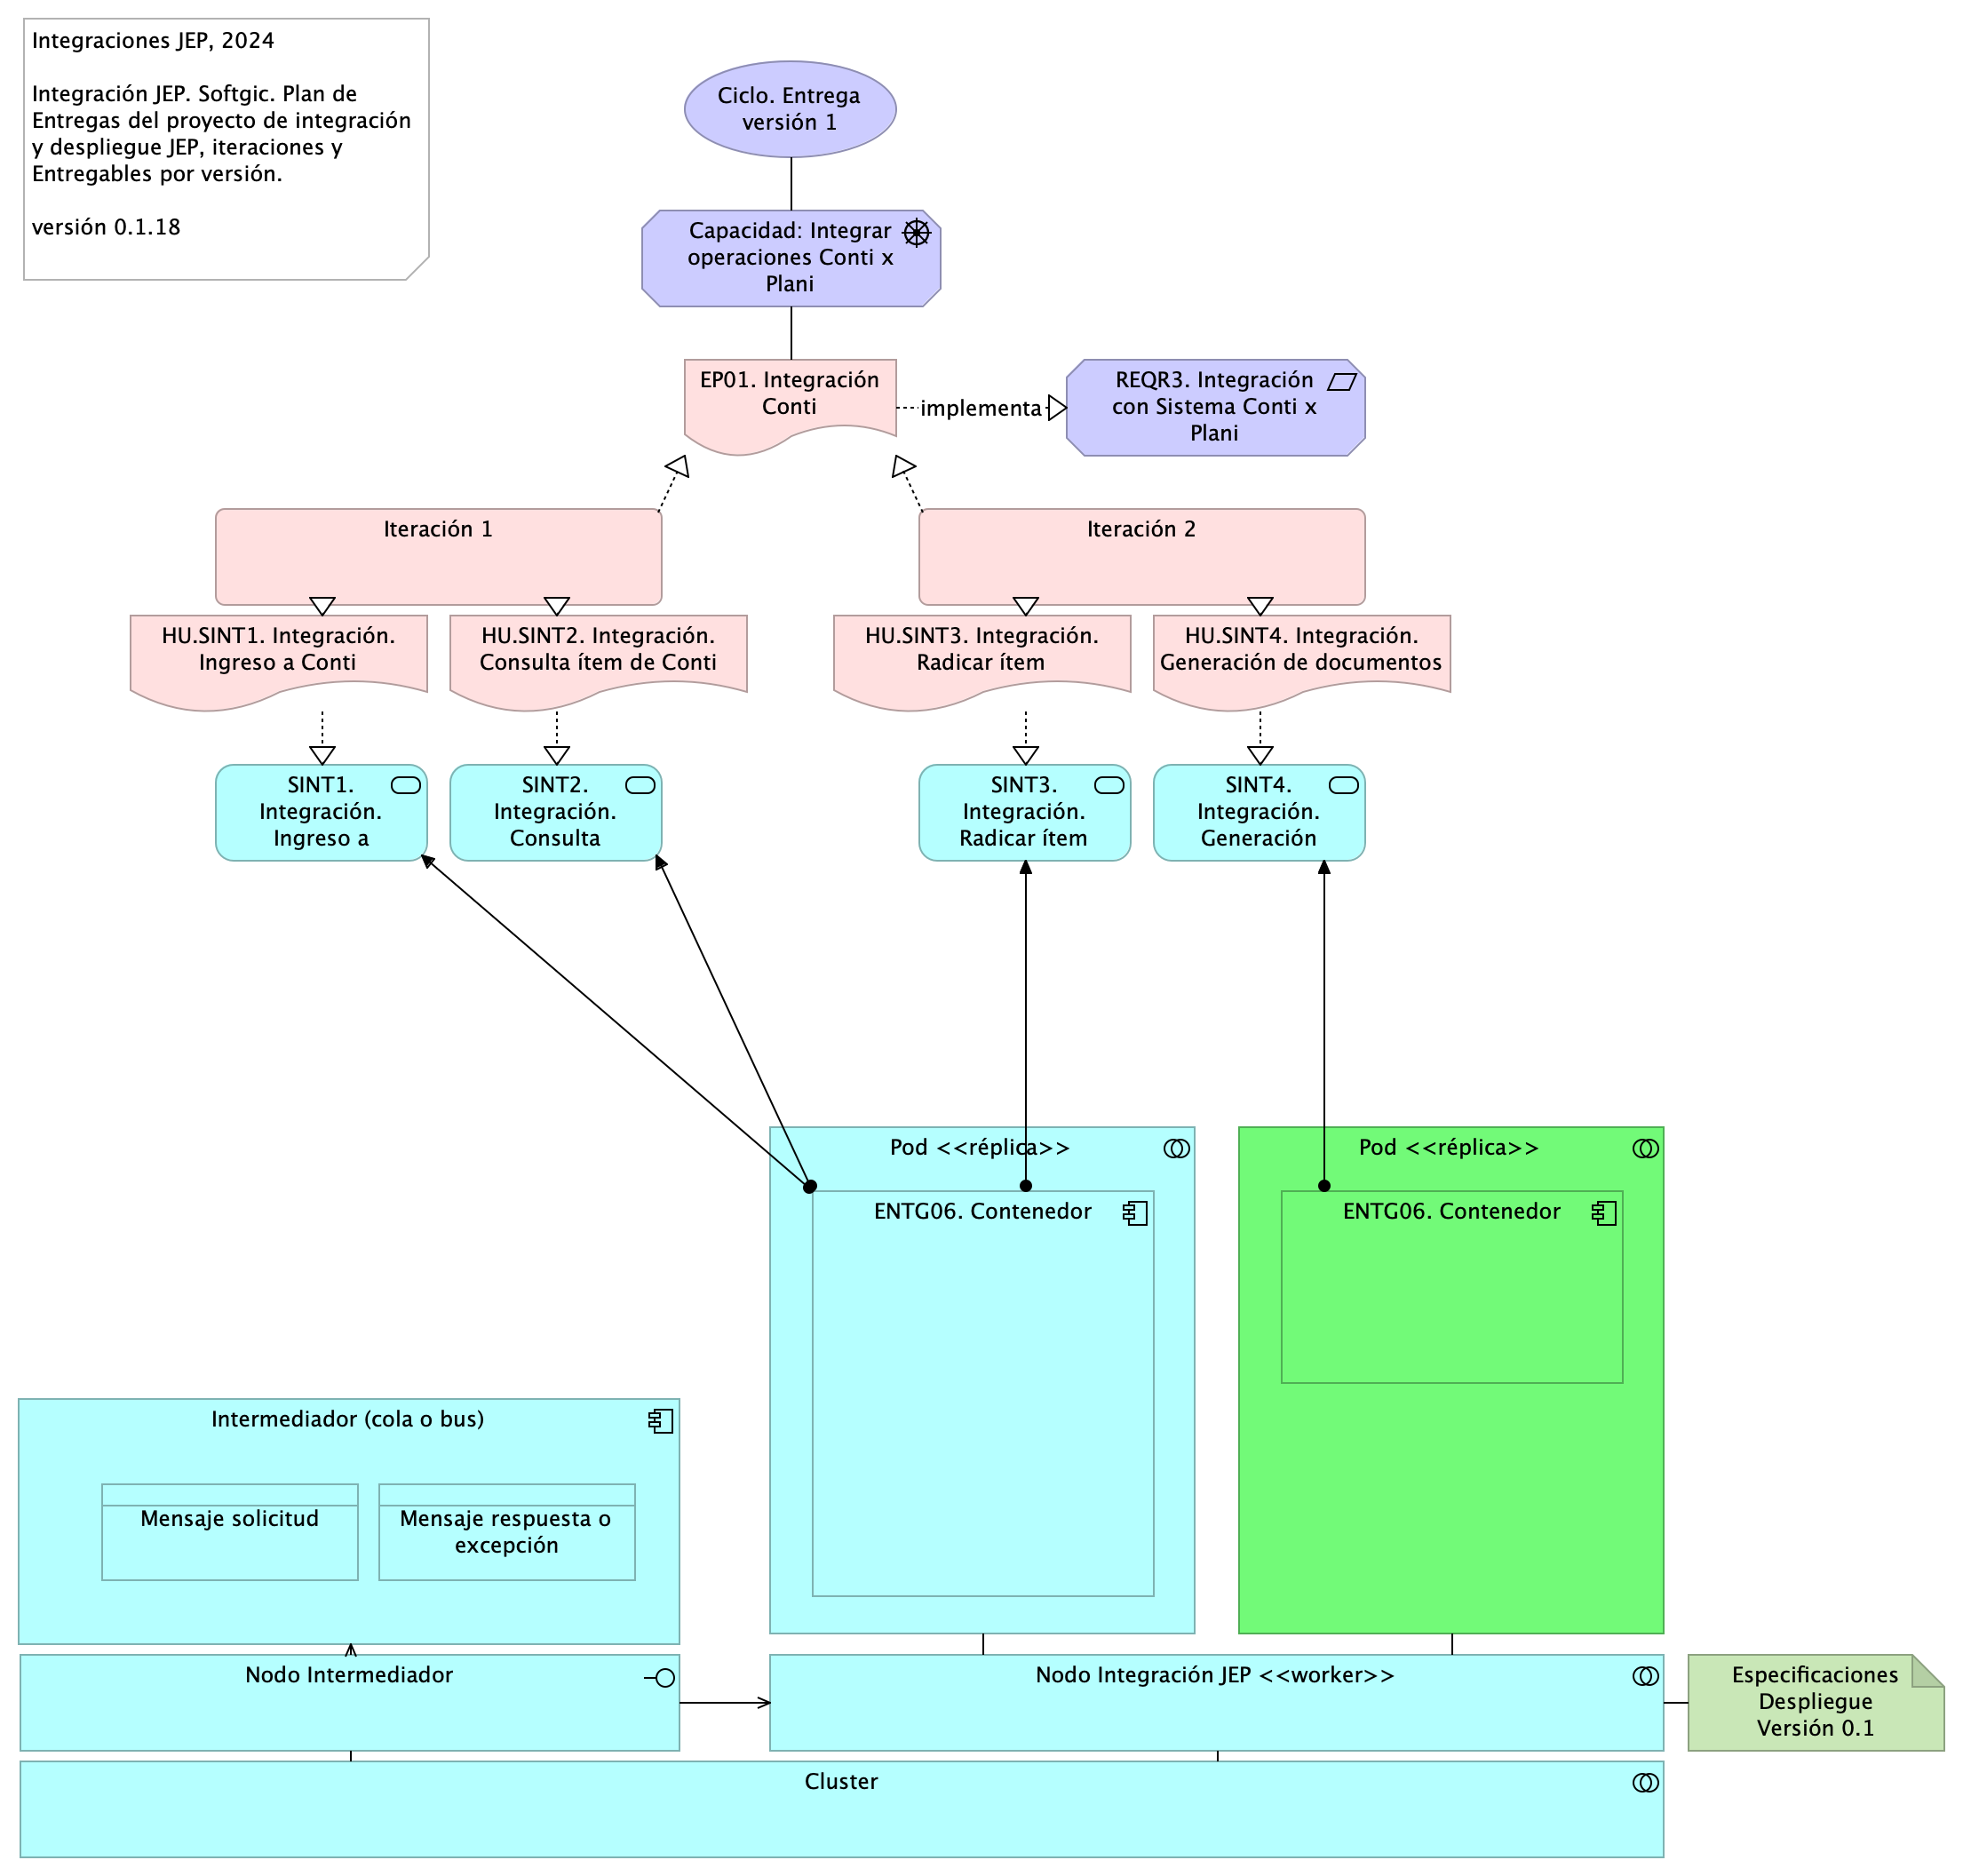
\includegraphics[width=\textwidth,height=5.20833in]{images/06.ENTRG.1n.1a.1.DespliegueEntregasdeRequerimientoVersion0.1.png}
\caption{06.ENTRG.1n.1a.1. Despliegue Entregas de Requerimiento Version
0.1. \emph{Fuente: Repositorio arquitectura Integración JEP
(2024)}}\label{fig:id-203e737545e449e59334b47d3034d956}
\end{figure}

\subsubsection{Catálogo de
Elementos}\label{sec:catuxe1logo-de-elementos-2}

\begin{longtable}[]{@{}
  >{\raggedright\arraybackslash}p{(\columnwidth - 4\tabcolsep) * \real{0.3000}}
  >{\raggedright\arraybackslash}p{(\columnwidth - 4\tabcolsep) * \real{0.2000}}
  >{\raggedright\arraybackslash}p{(\columnwidth - 4\tabcolsep) * \real{0.5000}}@{}}
\toprule\noalign{}
\begin{minipage}[b]{\linewidth}\raggedright
Nombre
\end{minipage} & \begin{minipage}[b]{\linewidth}\raggedright
Tipo
\end{minipage} & \begin{minipage}[b]{\linewidth}\raggedright
Documentación
\end{minipage} \\
\midrule\noalign{}
\endhead
\bottomrule\noalign{}
\endlastfoot
Capacidad: Integrar operaciones Conti & Driver & Característica de
integración de Conti contenido en la solución de integración JEP,
2024. \\
& & \\
Integración Conti & Deliverable & Épica de entrega de la solución de
integración JEP, 2024, que contiene las iteraciones que realizarán la
característica `Integrar operaciones Conti'. \\
\end{longtable}

\textbar{} \textbar{} REQR3. Integración con Sistema Conti x Plani
\textbar{} Requirement \textbar{} Atendiendo la necesidad de la
Subdirección de Contratación de implementar el flujo de gestión
precontractual en el sistema de Gestión Documental - Conti se requiere
integrar con la información de los ítems del Plan Anual de Adquisiciones
-- PAA para iniciar el proceso, la cual se encuentra gestionada en el
Sistema de Gestión y Planeación Institucional PLANi.

Fuente: Acta de requerimientos Integración Plani - Proceso
Precontractual\_V4 (pdf).

\paragraph{Índice de la documentación (casos de
uso)}\label{sec:uxedndice-de-la-documentaciuxf3n-casos-de-uso-4}

\begin{enumerate}
\def\labelenumi{\arabic{enumi}.}
\tightlist
\item
  Integración. Ingreso a Conti
\item
  Integración. Consulta ítem de Conti
\item
  Integración. Radicar ítem
\item
  Integración. Generación de documentos
\end{enumerate}

\textbar{} \textbar{} SINT1. Integración. Ingreso a Conti \textbar{}
Application Service \textbar{} Tareas de desarrollo

\begin{itemize}
\item
  Interoperabilidad IOP1. Transporte / Entrega Consulta Negocio
\item
  Modelo de datos (XML, RBDMS, \ldots)
\item
  Esquema de datos (XSD, DTD, JSON-E\ldots)
\item
  Contratos de interoperabilidad (WSDL, API\ldots)
\item
  Mensajes petición IN (API, XML\ldots)
\item
  Mensajes respuesta OUT (API, XML\ldots)
\item
  Mensajes excepción (API, XML\ldots)
\item
  Transporte (REST, SOAP)
\item
  Función lógica (JEE, \ldots)
\item
  Registro y envío de actividad \textbar{} \textbar{} SINT2.
  Integración. Consulta ítem de Conti \textbar{} Application Service
  \textbar{} Tareas de desarrollo
\item
  Interoperabilidad IOP1. Transporte / Entrega Consulta Negocio
\item
  Modelo de datos (XML, RBDMS, \ldots)
\item
  Esquema de datos (XSD, DTD, JSON-E\ldots)
\item
  Contratos de interoperabilidad (WSDL, API\ldots)
\item
  Mensajes petición IN (API, XML\ldots)
\item
  Mensajes respuesta OUT (API, XML\ldots)
\item
  Mensajes excepción (API, XML\ldots)
\item
  Transporte (REST, SOAP)
\item
  Función lógica (JEE, \ldots)
\item
  Registro y envío de actividad \textbar{} \textbar{} SINT3.
  Integración. Radicar ítem \textbar{} Application Service \textbar{}
  Tareas de desarrollo
\item
  Interoperabilidad IOP1. Transporte / Entrega Consulta Negocio
\item
  Modelo de datos (XML, RBDMS, \ldots)
\item
  Esquema de datos (XSD, DTD, JSON-E\ldots)
\item
  Contratos de interoperabilidad (WSDL, API\ldots)
\item
  Mensajes petición IN (API, XML\ldots)
\item
  Mensajes respuesta OUT (API, XML\ldots)
\item
  Mensajes excepción (API, XML\ldots)
\item
  Transporte (REST, SOAP)
\item
  Función lógica (JEE, \ldots)
\item
  Registro y envío de actividad \textbar{} \textbar{} SINT4.
  Integración. Generación de documentos \textbar{} Application Service
  \textbar{} Tareas de desarrollo
\item
  Interoperabilidad IOP1. Transporte / Entrega Consulta Negocio
\item
  Modelo de datos (XML, RBDMS, \ldots)
\item
  Esquema de datos (XSD, DTD, JSON-E\ldots)
\item
  Contratos de interoperabilidad (WSDL, API\ldots)
\item
  Mensajes petición IN (API, XML\ldots)
\item
  Mensajes respuesta OUT (API, XML\ldots)
\item
  Mensajes excepción (API, XML\ldots)
\item
  Transporte (REST, SOAP)
\item
  Función lógica (JEE, \ldots)
\item
  Registro y envío de actividad \textbar{} \textbar{} ENTG06. Contenedor
  \textbar{} Application Component \textbar{} Contenedores de los
  servicios de integración del proyecto desplegados en la
  infraestructura tecnológica JEP. \textbar{} \textbar{} ENTG06.
  Contenedor \textbar{} Application Component \textbar{} Contenedores de
  los servicios de integración del proyecto desplegados en la
  infraestructura tecnológica JEP. \textbar{} \textbar{} Intermediador
  (cola o bus) \textbar{} Application Component \textbar{} Bus de Red
  Hat, aplicación cliente Quarkus, o intermediador de integración Apache
  Camel. \textbar{} \textbar{} Mensaje solicitud \textbar{} Data Object
  \textbar{} Formato predefinido de intercambio de datos. \textbar{}
  \textbar{} Mensaje respuesta o excepción \textbar{} Data Object
  \textbar{} Formato predefinido de intercambio de datos. \textbar{}
  \textbar{} Nodo Intermediador \textbar{} Application Interface
  \textbar{} Nodo lógico en donde corren los contenedores. \textbar{}
  \textbar{} Nodo Integración JEP (worker) \textbar{} Application
  Collaboration \textbar{} Nodo lógico en donde corren los contenedores.
  \textbar{} \textbar{} Especificaciones Despliegue Versión 0.1
  \textbar{} Artifact \textbar{} \textbf{Documentación Técnica:
  Configuración y Despliegue en JEP sobre OpenShift}
\end{itemize}

\textbf{1. Introducción}

El presente documento describe las configuraciones requeridas y las
consideraciones técnicas para los despliegues en el clúster de la JEP en
OpenShift. Este clúster está configurado con Service Mesh y utiliza
Istio para habilitar capacidades de observabilidad, gestión de tráfico y
seguridad. A continuación, se presentan las configuraciones clave, las
características del clúster y ejemplos relevantes.

\textbf{2. Configuración del Clúster de OpenShift}

Este clúster de OpenShift incluye características específicas que
condicionan el despliegue de aplicaciones:

\textbf{Características generales:}

\begin{itemize}
\tightlist
\item
  \textbf{Acceso:} La consola se encuentra en
  \url{https://console-openshift-console.apps.interopera.jep.gov.co/k8s/cluster/projects}.
\item
  \textbf{VPN:} Gateway Remoto: 190.144.149.224.
\item
  \textbf{Nodo asignado:} El nodo para los despliegues:
  \textbf{votan.interopera.jep.gov.co}.
\item
  \textbf{Entorno de Despliegue:} desarrollo-sg
\item
  \textbf{Inyección de sidecars mediante Istio:} Configurada por
  namespace con la anotación istio-injection: enabled
\end{itemize}

\textbf{Configuraciones del entorno:}

\begin{itemize}
\tightlist
\item
  \textbf{Service Mesh habilitado:} Gestionado por Istio, para el marco
  de enrutamiento y proxy del tráfico entre servicios.
\item
  \textbf{Istio Injection:} Activado a nivel del namespace
  \textbf{desarrollo-sg} con la anotación:
\end{itemize}

\begin{verbatim}
istio-injection: enabled
\end{verbatim}

Esta configuración permite que un sidecar sea inyectado automáticamente
en los Pods dentro del namespace.

\textbf{3. Consideraciones de Configuración}

\textbf{Inyección de Sidecar (Istio Injection):}

La inyección de sidecar es fundamental para integrar los Pods en el
Service Mesh. Para habilitarla, se debe incluir la siguiente anotación
en los Pods y configurarla a nivel de namespace:

\begin{verbatim}
annotations:

sidecar.istio.io/inject: "true"
\end{verbatim}

\textbf{Asignación de Nodo Específico:}

Para garantizar que los Pods se ejecuten en el nodo asignado
(votan.interopera.jep.gov.co), se debe agregar el siguiente fragmento en
la especificación del Pod:

\begin{verbatim}
nodeSelector:

kubernetes.io/hostname: votan.interopera.jep.gov.co
\end{verbatim}

\textbf{Configuración del Service:}

El Service Mesh requiere un Service que defina claramente los puertos y
protocolos que se exponen. Por ejemplo:

\begin{verbatim}
spec:

selector:

app: ejemplo-app

ports:

\- protocol: TCP

port: 9000

targetPort: 9000
\end{verbatim}

No es necesario definir el tipo de servicio ``type:
LoadBalancer/ClusterIP'' ya que con el Service Mesh habilitado, la
configuración entre servicios se gestiona internamente a través del
proxy sidecar (controlado por Istio). Este proxy opera sobre los
servicios internos tipo ClusterIP.

\textbf{4. Ejemplo de Configuraciones Importantes}

\textbf{Fragmento de Deployment:}

Incluye configuraciones críticas como la inyección de Istio,
restricciones de recursos y selección del nodo:

\begin{verbatim}
metadata:

annotations:

sidecar.istio.io/inject: "true"

spec:

nodeSelector:

kubernetes.io/hostname: votan.interopera.jep.gov.co

containers:

\- resources:

requests:

memory: "20Mi"

cpu: "100m"

limits:

memory: "80Mi"

cpu: "120m"
\end{verbatim}

\textbf{Fragmento de Service:}

Define el puerto y el protocolo para la comunicación del Pod:

\begin{verbatim}
spec:

ports:

\- protocol: TCP

port: 9000

targetPort: 9000

selector:


app: ejemplo-app
\end{verbatim}

\textbf{5. Limitaciones del Entorno}

\begin{enumerate}
\def\labelenumi{\arabic{enumi}.}
\tightlist
\item
  \textbf{Dependencia del Service Mesh:}\\
  Todos los Pods deben estar configurados adecuadamente para aprovechar
  el Service Mesh. Un error en la configuración podría provocar
  problemas de conectividad o trazabilidad.
\item
  \textbf{Recursos restringidos:}\\
  Los límites de memoria y CPU deben ser estrictamente respetados para
  evitar conflictos de recursos en el clúster.
\item
  \textbf{Asignación de nodo fijo:}\\
  Aunque garantiza estabilidad, la dependencia de un nodo específico
  puede ser una desventaja si el nodo no está disponible.
\end{enumerate}

\textbf{6. Conclusión}

El clúster de OpenShift descrito está configurado para gestionar
aplicaciones bajo un marco controlado, con Service Mesh e Istio como
componentes clave. Las configuraciones presentadas aseguran que los
despliegues cumplan con los estándares definidos, aunque es fundamental
monitorear y ajustar según las necesidades específicas para el proyecto.
\textbar{} \textbar{} Cluster \textbar{} Application Collaboration
\textbar{} Orquestador de nodos y servicios (contendores) de la JEP.
\textbar{}

Table: Elementos de la vista.
\{\#tbl:tblelement-06.ENTRG.1n.1a.1.DespliegueEntregasdeRequerimientoVersion0.1-id\}

\subsection{Plantilla de Casos de Uso del Proyecto
JEP}\label{sec:plantilla-de-casos-de-uso-del-proyecto-jep}

\begin{figure}
\centering
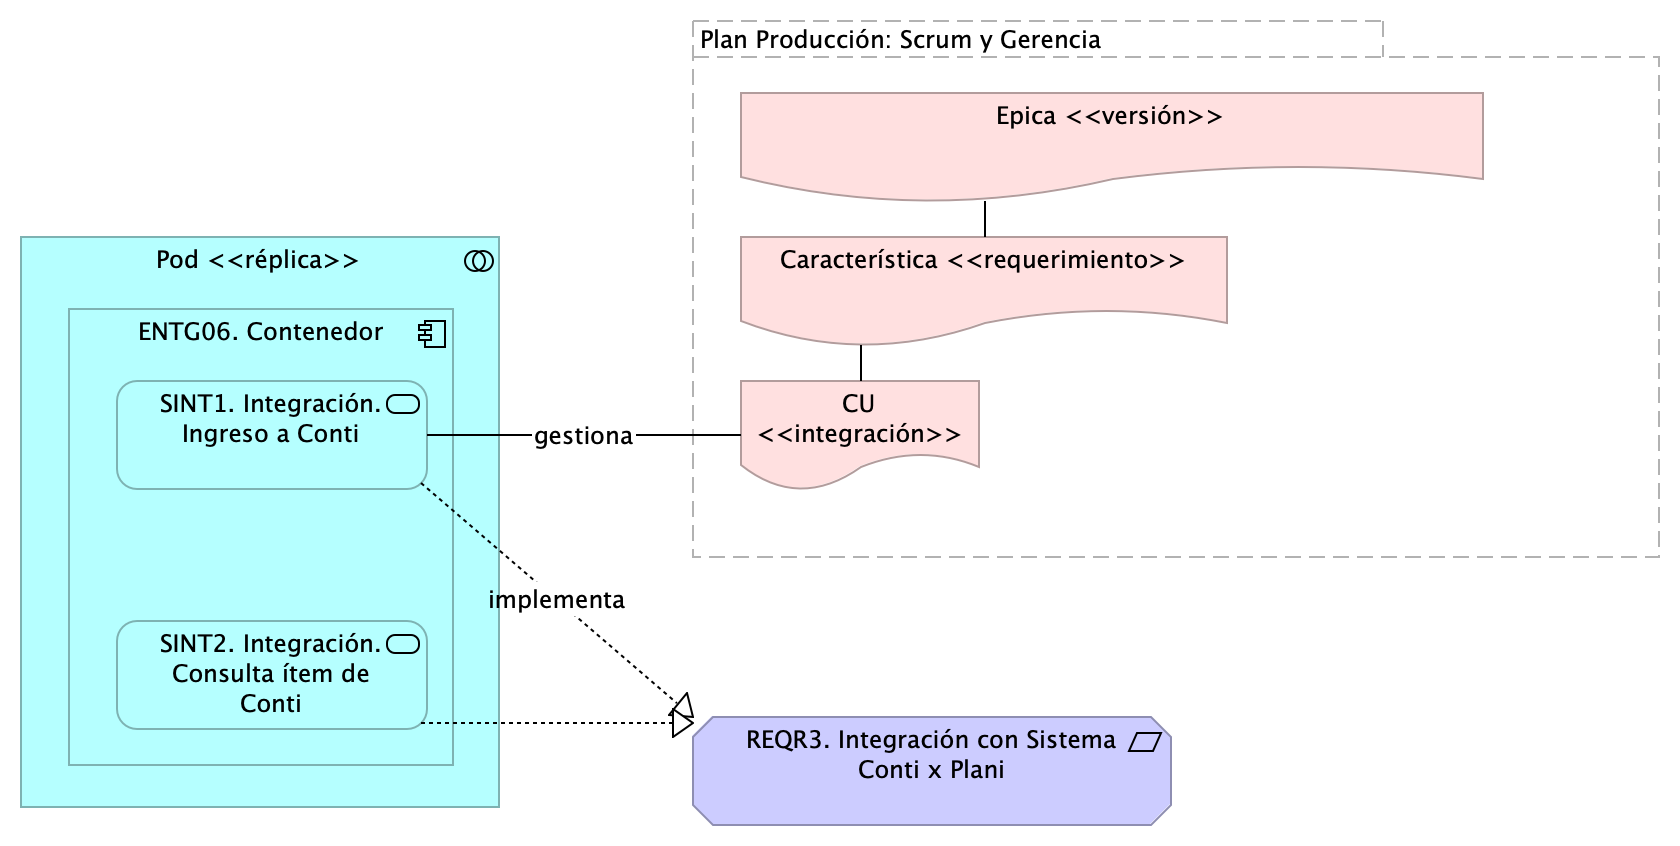
\includegraphics[width=\textwidth,height=5.20833in]{images/05.REQR.1n.3n.PlantillaCasodeUso.png}
\caption{05.REQR.1n.3n. Plantilla Caso de Uso. \emph{Fuente: Repositorio
arquitectura Integración JEP
(2024)}}\label{fig:id-8115cb4314954a7cb873b534038c22aa}
\end{figure}

Documentación de los casos de uso de integración (CU en el diagrama) del
proyecto JEP relacionados con las integraciones y requerimientos.

Fuente: Justificativo de la Contratación Invitación Pública.

\subsection{Casos de Uso del Proyecto
(integración)}\label{sec:casos-de-uso-del-proyecto-integraciuxf3n}

App A requiere integrar Información {[}I{]} \textbar{} Funcionalidad
{[}F{]} \textbar{} Servicios {[}S{]} con la App B, C, D\ldots{}

\subsubsection{Elementos}\label{sec:elementos-4}

Elegir y describir los elementos de la actual integración.

\begin{itemize}
\tightlist
\item[$\square$]
  App consumidora (A)
\item[$\square$]
  Mensaje
\item[$\square$]
  Canal
\item[$\square$]
  Ruteo
\item[$\square$]
  Traducción
\item[$\square$]
  App proveedora (B)
\item[$\square$]
  Monitoreo
\end{itemize}

\subsubsection{Diseño}\label{sec:diseuxf1o-4}

Message Construct \textbar{} Message Routing \textbar{} Message
Transformation \textbar{} Messaging Endpoints \textbar{} Messaging
Channels \textbar{} \ldots{}

\subsubsection{Matriz de
interoperabilidad}\label{sec:matriz-de-interoperabilidad-4}

Detalle del intercambio entre sistemas de información o aplicaciones.

Sistema A comparte información, funcionalidad o servicios con Sistema B.

\begin{longtable}[]{@{}lllll@{}}
\toprule\noalign{}
& Conti & Plani & Legali & Otros \\
\midrule\noalign{}
\endhead
\bottomrule\noalign{}
\endlastfoot
Conti & X & Inf, Seguridad & & \\
Plani & & X & & \\
Legali & & & X & \\
Otros Sistemas & & & & X \\
\end{longtable}

\subsubsection{Pruebas Realizables}\label{sec:pruebas-realizables-4}

Describir por cada caso de prueba de integración el resultado del
intercambio entre sistemas de información o aplicaciones según la Matriz
de interoperabilidad.

\end{document}
